% ===========================================================================
% Simulation study. Included from main.tex with % ===========================================================================
% Simulation study. Included from main.tex with % ===========================================================================
% Simulation study. Included from main.tex with % ===========================================================================
% Simulation study. Included from main.tex with \input{simulation}.
% Every number comes from paper/sim/*.tex and every figure from
% paper/sim/fig-*.pdf, generated by
%   cd libqueuingsim && cargo run --release --example paper_tables
%   uv run ... python scripts/plot_sim.py
% scripts/check_sim.sh fails if the generated files are stale.
% ===========================================================================
\input{sim/macros}

\subsection{Uncalibrated Simulation}\label{sec:sim}

The propositions hold inside their model. This subsection asks two
further questions by discrete-event simulation: does a simulation that
satisfies a proposition's assumptions reproduce its closed form, and
when an assumption is dropped, does the decision the proposition implies
survive? The simulator is not calibrated. Its parameters are
illustrative, and every number below is a property of the simulated
model under a synthetic workload. None is a measurement of a serving
system, and none replaces an entry of \S\ref{sec:exp-real}.

\paragraph{Simulator.} \texttt{libqueuingsim} is an event-driven
simulator written in Rust with six models: an open G/G/$c$ FIFO queue,
cross-checked against Lindley's recursion; closed agent programs on a
single-turn replica with a finite KV pool; the two-resource replica of
\S\ref{sec:batch}, fed by Poisson sessions with the closed turn/tool
loop of \S\ref{sec:sessions}; offline eviction instances with an exact
dynamic-programming optimum; disaggregated pools (kept for a follow-up);
and replicas with per-program KV locality. The two-resource replica runs
iterations of length $\max(\omega+\beta K_B,\ n\,a)$ for a batch of $n$
decoding turns holding $K_B$ tokens of KV, so decode is a bandwidth PS
with the demand~\eqref{eq:decode} and prefill is a FIFO server that
receives the compute the batch leaves. Resident KV is a prefix; a turn
re-prefills what was evicted with the work~\eqref{eq:prefill}. We use
$a=2\cdot10^{-5}$, $b=2\cdot10^{-9}$, $\omega=2\cdot10^{-4}$ and, in
the open-session scenario, $\beta=2\cdot10^{-9}$ seconds per token.
Whether a program issues another turn is drawn when its tool call
returns, so a suspended program holds KV that may never be reused.

\paragraph{Checks.} Each proposition is a named check with fixed seeds
and an explicit tolerance. An \emph{in-model} check keeps the
proposition's assumptions, so a failure would indicate a bug in the
simulator or in the closed form. A \emph{beyond-model} check drops one:
a real batch cap, a hit rate that emerges from finite memory, or a
heuristic in place of the optimum. Offloading checks on the single-turn
replica are in the code but not shown; their one finding, that the
ranking of offloading policies flips with whether fetches hold the
replica, is recorded for E3. Of \simChecks{} checks,
\simChecksPassed{} pass. Confidence intervals are 95\,\% batch means or,
where stated, across independent seeds. Every table and figure in this
subsection is generated by the simulator from fixed seeds; the best
value in each comparison is in bold.

\input{sim/tab-inmodel}
\input{sim/tab-ps}

\subsubsection{In-Model: The Closed Forms}\label{sec:sim-inmodel}

Table~\ref{tab:sim-inmodel} compares the closed forms of
\S\ref{sec:congestion} and the price of a miss with simulation under
their own assumptions; the M/M/1 response time, the PK wait, the
variance ratio, the $(1+\mathrm{CV}^2)/2$ ratio of Eq.~\eqref{eq:cv2}
and the worst shortest-first ratio over 9000 instances agree with theory
within the confidence interval or 2\,\%. The $\Delta L$ row forces
misses on a fraction $\delta$ of turns at an M/G/1 server; the rise in
the number of turns lies inside the bracket of
Proposition~\ref{prop:price}(i), at its upper end where the exact PK
difference lies. Table~\ref{tab:sim-ps} does the same for the replica.
Under PS, deterministic and hit/miss work of equal mean give the same
occupancy, as insensitivity says, while a FIFO server separates them as
Eq.~\eqref{eq:pk} predicts. With Poisson sessions, a closed turn/tool
loop and hyperexponential tool times (the ``Loop'' rows), a PS replica
matches the isolated formula at the turn rate $\lambda=\Lambda/(1-p)$,
as the product form says. On the two-resource replica, forced misses
raise the prefill queue by an amount inside the bracket of
Proposition~\ref{prop:price} and leave the decode batch unchanged, as
Proposition~\ref{prop:decode} says; the prefill server's availability
was $0.96$ in this run, so the M/G/1 approximation of the prefill stage
is close. A Monte Carlo of the admission counts of
\S\ref{sec:batch} reproduces $2$, $7/4$, $1$ and $95/64$
to three decimals. These checks confirm the simulator, not the
propositions, which are already proved.

\subsubsection{Beyond the Model}\label{sec:sim-beyond}

\input{sim/tab-lps}

\paragraph{A real batch cap.} The model treats the batch limit $B$ by
flattening $\varphi$ at $B$, which keeps the decode stage insensitive. A
real cap admits turns beyond $B$ in FIFO order. Table~\ref{tab:sim-lps}
and Figure~\ref{fig:sim-lps} compare the two. At half load they agree
within 1\,\% for every work law, and for exponential work at every load.
At high load the error follows the work $\mathrm{CV}^2$: for
deterministic work the capped replica holds fewer turns than the formula
(by 22\,\% at $u=0.9$), for hyperexponential work with $\mathrm{CV}^2=4$
it holds more (by 51\,\%). A capped batch is not insensitive, and since
hit/miss work has $\mathrm{CV}^2>1$, the model underestimates decode
congestion at a capped replica near saturation. E1 and E2 must report
which regime a deployment is in.

\begin{figure}[t]
\centering
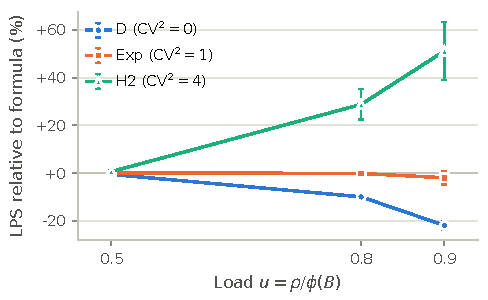
\includegraphics[width=\columnwidth]{sim/fig-lps}
\caption{Error of the saturating-$\varphi$ formula against an exact
batch cap ($B=8$) as a function of load, one line per work law. The
sign follows the work $\mathrm{CV}^2$. Synthetic, uncalibrated.}
\label{fig:sim-lps}
\end{figure}

\input{sim/tab-evict}

\paragraph{Eviction offline.} Table~\ref{tab:sim-evict} and
Figure~\ref{fig:sim-evict} score eviction rules against the exact
optimum on random instances. With equal $p_i$, shortest-first and
price-per-byte order choose the same programs and stay within a factor
of~2 of the optimum, as Proposition~\ref{prop:blind}(ii) requires. When
$p_i$ varies, shortest-first reaches ten times the optimum and the
price-per-byte order stays close; the guarded rule of
Proposition~\ref{prop:guarded} is within $1.9$ of the optimum on every
instance and has the lowest mean in every row. With prices unrelated to
size, plain program-level order reaches $6.7$ times the optimum on
random instances, and the adversarial family of
Proposition~\ref{prop:guarded}(i) makes it arbitrarily bad. At block
granularity the threshold rule equals the optimum on every instance and
the density prefix plus one block never exceeds the optimum by more
than that block's price, as Proposition~\ref{prop:memory} states.

\begin{figure}[t]
\centering
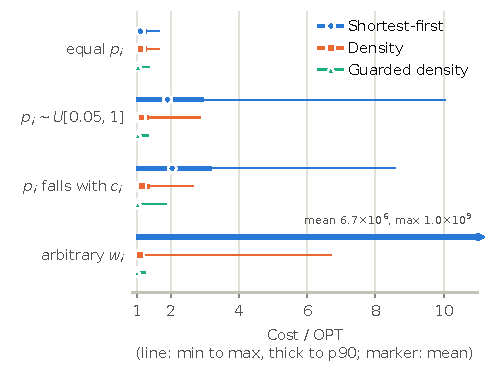
\includegraphics[width=\columnwidth]{sim/fig-evict-offline}
\caption{Offline eviction cost relative to the exact optimum by rule
and regime (mean, with the worst instance marked). Synthetic,
uncalibrated.}
\label{fig:sim-evict}
\end{figure}

\input{sim/tab-evict-dyn}
\input{sim/tab-admission}

\paragraph{Open sessions and admission.} Tables~\ref{tab:sim-evict-dyn}
and~\ref{tab:sim-admission} and Figure~\ref{fig:sim-admission} run the
two-resource replica with Poisson sessions, half agents with long tool
calls and half one-shot documents with short think times, on a 600k-token
pool. Three things are visible. First, the price is paid in TTFT. The
p99 time to first token is ten to seventeen times its mean, because up
to eight admitted prefills queue behind a document miss, while turn
response exceeds TTFT by a constant decode time in every cell, as
Proposition~\ref{prop:decode} predicts; in this roofline model a batch
of eight is memory-bound and leaves prefill almost all of the compute.
Second, the byte-second key of Proposition~\ref{prop:memory}, which
drops documents with short think time and low resume probability first,
has the lowest TTFT and highest throughput of the priced rules in most
cells, but no cell separates it from shortest-first or from plain
price-per-byte order beyond the seed noise; LRU is worst everywhere, by
a factor of two or more in throughput. Third, admission decides more
than the eviction order. With at most 16 live sessions the hit rate
stays at $0.99$ and TTFT below $0.4$\,s at both loads; with 24 the hit
rate degrades to $0.77$ at the higher load; with 32 most seeds thrash
at the higher load, throughput falls by 40\,\% and TTFT reaches 15\,s.
The cost of a tight cap is the entry-queue wait, and at $\Lambda=0.28$
the replica does not carry the offered turn rate under any cap, so the
entry waits there are growth over the horizon, not steady state. The
simulation therefore points E4 at admission as much as at eviction, and
it suggests that the price of a state is dominated by the thrash it can
trigger, a transient effect outside the stationary
Propositions~\ref{prop:price} and~\ref{prop:decode}. These are
synthetic two-class results; we do not claim that they hold for real
traces.

\begin{figure}[t]
\centering
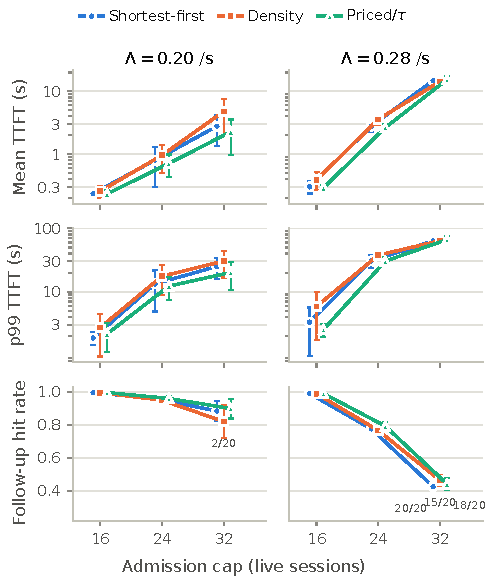
\includegraphics[width=\columnwidth]{sim/fig-admission}
\caption{Admission-cap sweep on the two-resource replica: mean and p99
time to first token and hit rate by cap and eviction rule at two session
arrival rates; annotations give the number of seeds (of 20) that
thrashed. Synthetic, uncalibrated.}
\label{fig:sim-admission}
\end{figure}

\input{sim/tab-inversion}

\paragraph{Placement and a shared KV store.} Table~\ref{tab:sim-inversion}
takes Proposition~\ref{prop:routing} out of its model: four replicas
instead of one node and an idle alternative, a skewed placement that
loads one replica, and a state that is moved over one shared link
rather than recomputed, as a shared KV store would move it. The row
order is the proposition's: the faster the link, the cheaper the move
and the lower the load at which always moving beats strict affinity.
With a link that moves a context in a millisecond the inversion is
below the lowest load swept; with a link slower than a recompute it
sits near saturation. The utilisation of the affinity node at the
inversion follows $\rho^*$ for cheap moves and exceeds it for the
expensive one, because the link is itself a shared resource: at the
loads where a slow link would pay off, every program is moving and the
link saturates, which the single-node proposition does not see. The
lookahead rule, which moves only when the observed wait exceeds the
move cost, is below both at every load, so the choice a deployment
faces is not affinity or a store but how the store's transfer is priced
at decision time.

\input{sim/tab-trace}

\paragraph{Replayed production sessions.} Table~\ref{tab:sim-trace}
replaces the synthetic classes by the production sessions of
\S\ref{sec:exp-traces}: sessions still arrive Poisson, but each one
replays a real session's appends, outputs, think times and length, so
the workload side of the model is measured and only the replica is
simulated. Three things follow. First, with no eviction every follow-up
turn hits and the prefill work still has
$\mathrm{CV}^2=\simTraceOpenCvMin$--$\simTraceOpenCvMax$, from the
appends alone; the mean TTFT is
\simTraceOpenTtftMin--\simTraceOpenTtftMax\,s at these loads because a
new session's first prompt, of a few hundred thousand tokens, is a
cold prefill that every turn behind it waits for. Second, once the pool
is finite the admission cap decides the regime. At the tight cap the
hit rate stays at or above \simTraceTightHitMin{} and the hit/miss
mixture supplies \simTraceTightMixMin--\simTraceTightMixMax\,\% of the
variance of follow-up prefill work, the split that E2 measures; at the
loose cap the replica thrashes, the hit rate falls to at most
\simTraceLooseHitMax{} and the mean TTFT exceeds
\simTraceLooseTtftMin\,s. The price of a tight cap is the entry wait,
up to \simTraceEntryMaxHours{} hours in the mean where the pool cannot
carry the offered sessions.
Third, the PK wait computed from the measured $\lambda$, $\E[S]$ and
$\E[S^2]$ of the prefill queue is above the observed wait in every cell,
by a factor of \simTracePkRatioMin{} to \simTracePkRatioMax. The live
sessions are a finite population of two to twenty-four, and a session
that is waiting cannot generate its next turn, so arrivals thin out as
the queue grows; the open M/G/1 queue of \S\ref{sec:batch} has no such
feedback and overstates the wait. The bracket of
Proposition~\ref{prop:price} is therefore conservative for small
populations, and E2 has to report the number of live sessions next to
the load.

\subsubsection{What the Simulation Does Not Show}\label{sec:sim-limits}

The simulator shares the model's abstractions. It does not model
block-level KV allocation beyond tail blocks, partial prefix hits
across sessions, collective-communication contention or a prefill
budget policy, and its replica has one capacity function for prefill
and decode. Its parameters were chosen to be plausible, not measured.
Its results show which decisions are robust to the assumptions we
dropped; they say nothing about how often each regime occurs in
practice. The experiments of \S\ref{sec:exp-real}, starting with the
calibration of E1, remain necessary.
.
% Every number comes from paper/sim/*.tex and every figure from
% paper/sim/fig-*.pdf, generated by
%   cd libqueuingsim && cargo run --release --example paper_tables
%   uv run ... python scripts/plot_sim.py
% scripts/check_sim.sh fails if the generated files are stale.
% ===========================================================================
% Generated by `uv run python -m report.paper_tables` in
% validation/. Do not edit by hand.
\newcommand{\simChecks}{35}
\newcommand{\simCalA}{0.194}
\newcommand{\simCalB}{6.51}
\newcommand{\simCalOmega}{0.057}
\newcommand{\simChecksPassed}{35}
\newcommand{\simDecodeShiftPct}{0.3}
\newcommand{\simEvictLruRatioMin}{1.0}
\newcommand{\simEvictLruRatioMax}{1.6}
\newcommand{\simEndUnknownHit}{0.59}
\newcommand{\simEndKnownHit}{1.00}
\newcommand{\simEndUnknownTtftRatio}{2.2}
\newcommand{\simPdAgree}{32}
\newcommand{\simPdCells}{32}
\newcommand{\simOffloadOk}{6}
\newcommand{\simOffloadCells}{6}
\newcommand{\simTracePkRatioMin}{4}
\newcommand{\simTracePkRatioMax}{12}
\newcommand{\simTraceOpenCvMin}{27}
\newcommand{\simTraceOpenCvMax}{38}
\newcommand{\simTraceOpenTtftMin}{62}
\newcommand{\simTraceOpenTtftMax}{208}
\newcommand{\simTraceTightHitMin}{0.59}
\newcommand{\simTraceTightReusedMin}{0.93}
\newcommand{\simTraceTightMixMin}{6}
\newcommand{\simTraceTightMixMax}{23}
\newcommand{\simTraceLooseHitMax}{0.66}
\newcommand{\simTraceLooseTtftMin}{966}
\newcommand{\simTraceSessions}{761}
\newcommand{\simTraceEntryMaxHours}{6}
\newcommand{\simPriceSmallRatioMin}{0.08}
\newcommand{\simPriceSmallRatioMax}{0.18}
\newcommand{\simPriceLargeRatioMin}{0.1}
\newcommand{\simPriceLargeRatioMax}{0.3}
\newcommand{\simPriceLiveMin}{2}
\newcommand{\simPriceLiveMax}{9}
\newcommand{\simPriceFiniteRatioMin}{3}
\newcommand{\simPriceFiniteRatioMax}{18}
\newcommand{\simPriceOverMin}{3}
\newcommand{\simPriceOverMax}{13}
\newcommand{\simPriceCapHolds}{every}
\newcommand{\simFiniteRatioMax}{4.5}
\newcommand{\simFiniteRatioMin}{1.09}
\newcommand{\simFiniteNMin}{2}
\newcommand{\simFiniteNMax}{64}
\newcommand{\simFiniteRho}{0.6}


\subsection{Uncalibrated Simulation}\label{sec:sim}

The propositions hold inside their model. This subsection asks two
further questions by discrete-event simulation: does a simulation that
satisfies a proposition's assumptions reproduce its closed form, and
when an assumption is dropped, does the decision the proposition implies
survive? The simulator is not calibrated. Its parameters are
illustrative, and every number below is a property of the simulated
model under a synthetic workload. None is a measurement of a serving
system, and none replaces an entry of \S\ref{sec:exp-real}.

\paragraph{Simulator.} \texttt{libqueuingsim} is an event-driven
simulator written in Rust with six models: an open G/G/$c$ FIFO queue,
cross-checked against Lindley's recursion; closed agent programs on a
single-turn replica with a finite KV pool; the two-resource replica of
\S\ref{sec:batch}, fed by Poisson sessions with the closed turn/tool
loop of \S\ref{sec:sessions}; offline eviction instances with an exact
dynamic-programming optimum; disaggregated pools (kept for a follow-up);
and replicas with per-program KV locality. The two-resource replica runs
iterations of length $\max(\omega+\beta K_B,\ n\,a)$ for a batch of $n$
decoding turns holding $K_B$ tokens of KV, so decode is a bandwidth PS
with the demand~\eqref{eq:decode} and prefill is a FIFO server that
receives the compute the batch leaves. Resident KV is a prefix; a turn
re-prefills what was evicted with the work~\eqref{eq:prefill}. We use
$a=2\cdot10^{-5}$, $b=2\cdot10^{-9}$, $\omega=2\cdot10^{-4}$ and, in
the open-session scenario, $\beta=2\cdot10^{-9}$ seconds per token.
Whether a program issues another turn is drawn when its tool call
returns, so a suspended program holds KV that may never be reused.

\paragraph{Checks.} Each proposition is a named check with fixed seeds
and an explicit tolerance. An \emph{in-model} check keeps the
proposition's assumptions, so a failure would indicate a bug in the
simulator or in the closed form. A \emph{beyond-model} check drops one:
a real batch cap, a hit rate that emerges from finite memory, or a
heuristic in place of the optimum. Offloading checks on the single-turn
replica are in the code but not shown; their one finding, that the
ranking of offloading policies flips with whether fetches hold the
replica, is recorded for E3. Of \simChecks{} checks,
\simChecksPassed{} pass. Confidence intervals are 95\,\% batch means or,
where stated, across independent seeds. Every table and figure in this
subsection is generated by the simulator from fixed seeds; the best
value in each comparison is in bold.

% Generated by `cargo run --release --example paper_tables` in
% libqueuingsim/. Do not edit by hand.
\begin{table}[t]
\caption{Simulation under each proposition's assumptions (in-model). M/M/1: $\mu=10$. PK: $\rho=0.7$. Cache: $\lambda=1.8$. SF/OPT: worst of 9000 instances with equal $p_i$. $\pm$ is a 95\,\% batch-means half-width. Times in seconds.}
\label{tab:sim-inmodel}
\centering\small
\begin{tabular}{@{}l@{\hspace{4pt}}lcc@{}}
\toprule
Quantity & Result & Theory & Simulated \\
\midrule
M/M/1 $W$, $\lambda=9$ & \S\ref{sec:intro} & 1.000 & $1.012 \pm 0.024$ \\
PK $W_q$, workload B & Thm.~\ref{thm:pk} & 4.002 & $3.960 \pm 0.052$ \\
$W_q^B/W_q^A$, $\rho=0.6$ & Prop.~\ref{prop:pk} & 3.43 & 3.42 \\
$\rho$ at $p=0.8$ & Prop.~\ref{prop:cache} & 0.252 & 0.253 \\
$W_q$ / M/M/1, $\mathrm{CV}^2{=}15.3$ & Eq.~\eqref{eq:cv2} & 8.15 & 8.10 \\
max SF/OPT & Prop.~\ref{prop:evict} & $\le 2$ & 1.791 \\
\bottomrule
\end{tabular}
\end{table}

% Generated by `cargo run --release --example paper_tables` in
% libqueuingsim/. Do not edit by hand.
\begin{table}[t]
\caption{Batching server under its assumptions (in-model): mean number of turns at the replica, $L=\lambda R$. Rows 1--4: Poisson turns at $\rho=0.7$, work deterministic or hit/miss ($0.05$\,s w.p.\ $0.8$, else $0.5$\,s; both mean $0.14$\,s); PS theory $\rho/(1-\rho)$, FIFO theory $\lambda W_q+\rho$. Rows 5--6: sessions arrive Poisson, each turn is followed by a tool call (mean 2\,s, $\mathrm{CV}^2=4$) and another turn w.p.\ $0.8$; theory $\sum_n n\pi(n)$ at $\lambda=\Lambda/(1-p)$ ($\rho=0.7$ for $\phi\equiv 1$, $\rho=3$ for $\phi(n)=n/(1+\beta(n-1))$). Row 7: rise of $L$ at a PS server when a fraction $\delta$ of turns becomes misses, hit rate $0.8$, $\rho=0.6$, against $[\lambda\delta\Phi_{\mathrm{PS}},\ \tfrac{C-\rho}{C-\rho'}\lambda\delta\Phi_{\mathrm{PS}}]$. Rows 8--9: the same misses on the two-resource replica (prefill FIFO in the compute left by a decode batch of $0.1$\,s per turn, mean availability $\bar r=0.96$): rise of the number in the prefill stage $L_P=\lambda\,\mathrm{TTFT}$ against the FIFO bracket at service $P/\bar r$, and of the number in the decode stage $L_D$, whose demand does not depend on hit or miss. $\pm$ is a 95\,\% batch-means half-width.}
\label{tab:sim-ps}
\centering\small\setlength{\tabcolsep}{3pt}
\begin{tabular}{@{}l@{\hspace{4pt}}lcc@{}}
\toprule
Quantity & Result & Theory & Simulated \\
\midrule
PS, D & \S\ref{sec:batch} & 2.333 & $2.338 \pm 0.021$ \\
PS, hit/miss & \S\ref{sec:batch} & 2.333 & $2.348 \pm 0.044$ \\
FIFO, D & Eq.~\eqref{eq:pk} & 1.517 & $1.519 \pm 0.011$ \\
FIFO, hit/miss & Eq.~\eqref{eq:pk} & 2.867 & $2.880 \pm 0.051$ \\
Loop, $\phi\equiv1$ & \S\ref{sec:sessions} & 2.33 & $2.36 \pm 0.07$ \\
Loop, sat.\ $\phi$ ($\beta{=}0.25$) & \S\ref{sec:sessions} & 12.00 & $12.32 \pm 0.39$ \\
PS $\Delta L$, $\delta{=}0.05$ & Prop.~\ref{prop:decode} & $[0.60,0.79]$ & $0.775 \pm 0.018$ \\
2-stage $\Delta L_P$, $\delta{=}0.05$ & Prop.~\ref{prop:price} & $[0.81,1.11]$ & $1.068 \pm 0.029$ \\
2-stage $\Delta L_D$, $\delta{=}0.05$ & Prop.~\ref{prop:decode} & 0 & $-0.000 \pm 0.000$ \\
\bottomrule
\end{tabular}
\end{table}


\subsubsection{In-Model: The Closed Forms}\label{sec:sim-inmodel}

Table~\ref{tab:sim-inmodel} compares the closed forms of
\S\ref{sec:congestion} and the price of a miss with simulation under
their own assumptions; the M/M/1 response time, the PK wait, the
variance ratio, the $(1+\mathrm{CV}^2)/2$ ratio of Eq.~\eqref{eq:cv2}
and the worst shortest-first ratio over 9000 instances agree with theory
within the confidence interval or 2\,\%. The $\Delta L$ row forces
misses on a fraction $\delta$ of turns at an M/G/1 server; the rise in
the number of turns lies inside the bracket of
Proposition~\ref{prop:price}(i), at its upper end where the exact PK
difference lies. Table~\ref{tab:sim-ps} does the same for the replica.
Under PS, deterministic and hit/miss work of equal mean give the same
occupancy, as insensitivity says, while a FIFO server separates them as
Eq.~\eqref{eq:pk} predicts. With Poisson sessions, a closed turn/tool
loop and hyperexponential tool times (the ``Loop'' rows), a PS replica
matches the isolated formula at the turn rate $\lambda=\Lambda/(1-p)$,
as the product form says. On the two-resource replica, forced misses
raise the prefill queue by an amount inside the bracket of
Proposition~\ref{prop:price} and leave the decode batch unchanged, as
Proposition~\ref{prop:decode} says; the prefill server's availability
was $0.96$ in this run, so the M/G/1 approximation of the prefill stage
is close. A Monte Carlo of the admission counts of
\S\ref{sec:batch} reproduces $2$, $7/4$, $1$ and $95/64$
to three decimals. These checks confirm the simulator, not the
propositions, which are already proved.

\subsubsection{Beyond the Model}\label{sec:sim-beyond}

% Generated by `uv run python -m report.paper_tables` in
% validation/. Do not edit by hand.
\begin{table}[htbp]
\caption{Batch cap $B=8$: exact limited PS (at most $B$ turns share $\phi(n)=n/(1+0.1(n-1))$, FIFO beyond) against PS with $\phi$ flattened at $B$, the model's approximation. Poisson turns, work of mean 1 with the given law ($\mathrm{CV}^2$ in brackets), load $u=\rho/\phi(B)$. Mean number at the replica; last column: relative error of the approximation for LPS, in \%. Mean response time has the same relative error (Little).}
\label{tab:sim-lps}
\centering\small\setlength{\tabcolsep}{3pt}
\begin{tabular}{@{}lccccc@{}}
\toprule
Work & $u$ & Formula & PS & LPS & Err. \\
\midrule
D (0) & 0.5 & 3.10 & $3.10 \pm 0.00$ & $3.08 \pm 0.00$ & $-1$ \\
D (0) & 0.8 & 7.33 & $7.33 \pm 0.06$ & $6.60 \pm 0.03$ & $-10$ \\
D (0) & 0.9 & 12.67 & $12.81 \pm 0.44$ & $9.90 \pm 0.22$ & $-22$ \\
Exp (1) & 0.5 & 3.10 & $3.11 \pm 0.01$ & $3.11 \pm 0.01$ & $+0$ \\
Exp (1) & 0.8 & 7.33 & $7.38 \pm 0.11$ & $7.38 \pm 0.11$ & $+1$ \\
Exp (1) & 0.9 & 12.67 & $12.73 \pm 0.52$ & $12.72 \pm 0.52$ & $+0$ \\
H2 (4) & 0.5 & 3.10 & $3.09 \pm 0.03$ & $3.12 \pm 0.03$ & $+1$ \\
H2 (4) & 0.8 & 7.33 & $7.29 \pm 0.18$ & $9.14 \pm 0.44$ & $+25$ \\
H2 (4) & 0.9 & 12.67 & $12.57 \pm 0.72$ & $20.31 \pm 1.87$ & $+60$ \\
\bottomrule
\end{tabular}
\end{table}


\paragraph{A real batch cap.} The model treats the batch limit $B$ by
flattening $\varphi$ at $B$, which keeps the decode stage insensitive. A
real cap admits turns beyond $B$ in FIFO order. Table~\ref{tab:sim-lps}
and Figure~\ref{fig:sim-lps} compare the two. At half load they agree
within 1\,\% for every work law, and for exponential work at every load.
At high load the error follows the work $\mathrm{CV}^2$: for
deterministic work the capped replica holds fewer turns than the formula
(by 22\,\% at $u=0.9$), for hyperexponential work with $\mathrm{CV}^2=4$
it holds more (by 51\,\%). A capped batch is not insensitive, and since
hit/miss work has $\mathrm{CV}^2>1$, the model underestimates decode
congestion at a capped replica near saturation. E1 and E2 must report
which regime a deployment is in.

\begin{figure}[t]
\centering
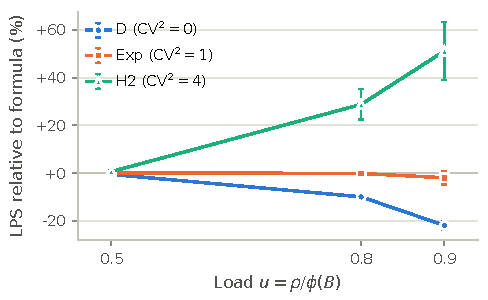
\includegraphics[width=\columnwidth]{sim/fig-lps}
\caption{Error of the saturating-$\varphi$ formula against an exact
batch cap ($B=8$) as a function of load, one line per work law. The
sign follows the work $\mathrm{CV}^2$. Synthetic, uncalibrated.}
\label{fig:sim-lps}
\end{figure}

% Generated by `cargo run --release --example paper_tables` in
% libqueuingsim/. Do not edit by hand.
\begin{table}[t]
\caption{Offline eviction: cost relative to the exact optimum of \eqref{eq:evict} with costs $p_ic_i^2$, over 3000 random instances per row (12 programs, $c_i\in\{1,\dots,200\}$, $\Delta C$ a random 10--60\,\% of the total).}
\label{tab:sim-evict}
\centering\small
\begin{tabular}{@{}lcccc@{}}
\toprule
Resume model & \multicolumn{2}{c}{SF mean / max} & \multicolumn{2}{c}{Density mean / max} \\
\midrule
equal $p_i$ & 1.108 & 1.67 & 1.108 & 1.67 \\
$p_i\sim U[0.05,1]$ & 1.902 & 10.05 & 1.136 & 2.86 \\
$p_i$ falls with $c_i$ & 2.037 & 8.60 & 1.146 & 2.67 \\
\bottomrule
\end{tabular}
\end{table}


\paragraph{Eviction offline.} Table~\ref{tab:sim-evict} and
Figure~\ref{fig:sim-evict} score eviction rules against the exact
optimum on random instances. With equal $p_i$, shortest-first and
price-per-byte order choose the same programs and stay within a factor
of~2 of the optimum, as Proposition~\ref{prop:blind}(ii) requires. When
$p_i$ varies, shortest-first reaches ten times the optimum and the
price-per-byte order stays close; the guarded rule of
Proposition~\ref{prop:guarded} is within $1.9$ of the optimum on every
instance and has the lowest mean in every row. With prices unrelated to
size, plain program-level order reaches $6.7$ times the optimum on
random instances, and the adversarial family of
Proposition~\ref{prop:guarded}(i) makes it arbitrarily bad. At block
granularity the threshold rule equals the optimum on every instance and
the density prefix plus one block never exceeds the optimum by more
than that block's price, as Proposition~\ref{prop:memory} states.

\begin{figure}[t]
\centering
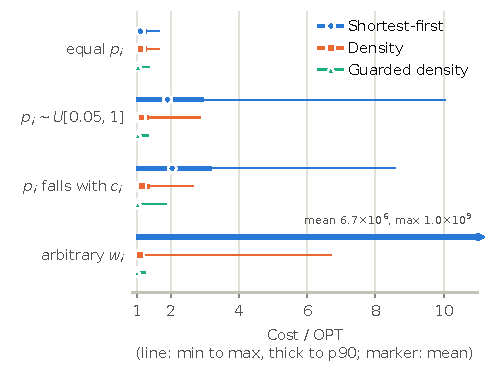
\includegraphics[width=\columnwidth]{sim/fig-evict-offline}
\caption{Offline eviction cost relative to the exact optimum by rule
and regime (mean, with the worst instance marked). Synthetic,
uncalibrated.}
\label{fig:sim-evict}
\end{figure}

% Generated by `uv run python -m report.paper_tables` in
% validation/. Do not edit by hand.
\begin{table}[htbp]
\caption{Eviction with open sessions on a replica with the vLLM~v1 engine's rules (those of Table~\ref{tab:sim-trace}) and the testbed's cost model. Sessions arrive Poisson at rate $\Lambda$ (per s): half agents ($p_i=0.95$, 4--8k initial tokens, tool calls Exp(6\,s)), half one-shot documents ($p_i=0.3$, 15--30k tokens, think time Exp(2\,s)); 600k-token KV, batch cap 8, at most 24 live sessions. Every policy evicts 16-token blocks from the tail of a context, sessions in a tool call before waiting ones (except LRU), and drops a finished session's blocks; rows marked $^*$ keep them, as vLLM's engine does, which cannot tell a finished session from one in a tool call. Throughput (turns/s), follow-up hit rate (the whole reusable prefix reused), mean and p99 time to first token (s), mean turn response (s; its half-width is in the data file), and the number of the 20 seeds that thrashed (follow-up turns reusing less than half of their reusable prefix); $\pm$ is a 95\,\% half-width over seeds; the best throughput, hit rate, TTFT and p99 per load in bold. Priced: $p_i\Phi_i/c_i$ with the FIFO price of Prop.~\ref{prop:price} from online estimates at the engine; Priced/$\tau$: per byte-second, $p_i\Phi_i/(c_i\tau_i)$ (the threshold rule of \S\ref{sec:evict}); Blocks: the same price of the tail block. The priced rules take $p_i$ and $\tau_i$ from the generating class (an oracle); the fixed keys see neither.}
\label{tab:sim-evict-dyn}
\centering\small\setlength{\tabcolsep}{2pt}
\begin{tabular}{@{}clcccccc@{}}
\toprule
$\Lambda$ & Policy & $X$ & Hit & TTFT & p99 & $R$ & Thr. \\
\midrule
0.03 & SF & \textbf{0.29} & \textbf{1.00} & $\mathbf{2.22 \pm 0.15}$ & \textbf{16.8} & 20.2 & 0 \\
0.03 & Density & \textbf{0.29} & \textbf{1.00} & $\mathbf{2.22 \pm 0.15}$ & \textbf{16.8} & 20.2 & 0 \\
0.03 & Priced & \textbf{0.29} & \textbf{1.00} & $\mathbf{2.22 \pm 0.15}$ & \textbf{16.8} & 20.2 & 0 \\
0.03 & Priced/$\tau$ & \textbf{0.29} & \textbf{1.00} & $\mathbf{2.22 \pm 0.15}$ & \textbf{16.8} & 20.2 & 0 \\
0.03 & Blocks & \textbf{0.29} & \textbf{1.00} & $\mathbf{2.22 \pm 0.15}$ & \textbf{16.8} & 20.2 & 0 \\
0.03 & LRU & \textbf{0.29} & \textbf{1.00} & $\mathbf{2.22 \pm 0.15}$ & \textbf{16.8} & 20.2 & 0 \\
0.03 & LRU$^*$ & \textbf{0.29} & \textbf{1.00} & $\mathbf{2.22 \pm 0.15}$ & \textbf{16.8} & 20.2 & 0 \\
0.03 & Priced/$\tau$$^*$ & \textbf{0.29} & 0.59 & $4.80 \pm 0.50$ & 29.3 & 23.6 & 0 \\
0.05 & SF & \textbf{0.38} & \textbf{0.83} & $34.45 \pm 1.01$ & 70.4 & 53.4 & 0 \\
0.05 & Density & \textbf{0.38} & \textbf{0.83} & $\mathbf{34.39 \pm 1.01}$ & \textbf{69.6} & 53.4 & 0 \\
0.05 & Priced & \textbf{0.38} & \textbf{0.83} & $34.48 \pm 0.99$ & 70.7 & 53.5 & 0 \\
0.05 & Priced/$\tau$ & \textbf{0.38} & \textbf{0.83} & $34.43 \pm 1.01$ & 70.4 & 53.4 & 0 \\
0.05 & Blocks & \textbf{0.38} & \textbf{0.83} & $34.46 \pm 1.00$ & 70.6 & 53.5 & 0 \\
0.05 & LRU & 0.27 & 0.75 & $56.41 \pm 1.76$ & 226.2 & 77.3 & 0 \\
0.05 & LRU$^*$ & 0.24 & 0.70 & $66.89 \pm 2.39$ & 240.9 & 88.2 & 0 \\
0.05 & Priced/$\tau$$^*$ & 0.35 & 0.45 & $41.73 \pm 0.68$ & 71.8 & 61.6 & 0 \\
\bottomrule
\end{tabular}
\end{table}

% Generated by `uv run python -m report.paper_tables` in
% validation/. Do not edit by hand.
\begin{table}[htbp]
\caption{Admission-cap sweep on the vLLM-rule replica: the scenario of Table~\ref{tab:sim-evict-dyn} with at most 16, 24 or 32 live sessions; later arrivals wait in an entry queue. Throughput (turns/s), follow-up hit rate, mean and p99 time to first token (s), mean turn response (s), mean entry-queue wait of a new session (s), and the number of the 20 seeds that thrashed. Means over seeds; the best throughput, hit rate, TTFT and p99 per ($\Lambda$, cap) in bold. The 95\,\% half-widths over seeds are the whiskers of Figure~\ref{fig:sim-admission}; Table~\ref{tab:sim-evict-dyn} states them for the rows it shares. An entry wait of hundreds of seconds means the replica does not carry the offered turn rate and the entry queue grows over the run; such values depend on the horizon (20\,000\,s). Every policy drops a finished session's blocks.}
\label{tab:sim-admission}
\centering\small\setlength{\tabcolsep}{2pt}
\begin{tabular}{@{}ccl@{\hspace{3pt}}cccccccc@{}}
\toprule
$\Lambda$ & Cap & Policy & $X$ & Hit & TTFT & p99 & $R$ & Entry & Thr. \\
\midrule
0.03 & 16 & SF & \textbf{0.29} & \textbf{1.00} & \textbf{2.21} & \textbf{16.5} & 20.20 & 0.1 & 0 \\
0.03 & 16 & Density & \textbf{0.29} & \textbf{1.00} & \textbf{2.21} & \textbf{16.5} & 20.20 & 0.1 & 0 \\
0.03 & 16 & Priced/$\tau$ & \textbf{0.29} & \textbf{1.00} & \textbf{2.21} & \textbf{16.5} & 20.20 & 0.1 & 0 \\
0.05 & 16 & SF & \textbf{0.41} & \textbf{1.00} & \textbf{14.54} & \textbf{33.5} & 32.89 & 1297.7 & 0 \\
0.05 & 16 & Density & \textbf{0.41} & \textbf{1.00} & \textbf{14.54} & \textbf{33.5} & 32.89 & 1297.7 & 0 \\
0.05 & 16 & Priced/$\tau$ & \textbf{0.41} & \textbf{1.00} & \textbf{14.54} & \textbf{33.5} & 32.89 & 1297.7 & 0 \\
0.03 & 24 & SF & \textbf{0.29} & \textbf{1.00} & \textbf{2.22} & \textbf{16.8} & 20.21 & 0.0 & 0 \\
0.03 & 24 & Density & \textbf{0.29} & \textbf{1.00} & \textbf{2.22} & \textbf{16.8} & 20.21 & 0.0 & 0 \\
0.03 & 24 & Priced/$\tau$ & \textbf{0.29} & \textbf{1.00} & \textbf{2.22} & \textbf{16.8} & 20.21 & 0.0 & 0 \\
0.05 & 24 & SF & \textbf{0.38} & \textbf{0.83} & 34.45 & 70.4 & 53.44 & 1407.5 & 0 \\
0.05 & 24 & Density & \textbf{0.38} & \textbf{0.83} & \textbf{34.39} & \textbf{69.6} & 53.38 & 1407.3 & 0 \\
0.05 & 24 & Priced/$\tau$ & \textbf{0.38} & \textbf{0.83} & 34.43 & 70.4 & 53.42 & 1408.4 & 0 \\
0.03 & 32 & SF & \textbf{0.29} & \textbf{1.00} & \textbf{2.22} & \textbf{16.8} & 20.21 & 0.0 & 0 \\
0.03 & 32 & Density & \textbf{0.29} & \textbf{1.00} & \textbf{2.22} & \textbf{16.8} & 20.21 & 0.0 & 0 \\
0.03 & 32 & Priced/$\tau$ & \textbf{0.29} & \textbf{1.00} & \textbf{2.22} & \textbf{16.8} & 20.21 & 0.0 & 0 \\
0.05 & 32 & SF & \textbf{0.32} & \textbf{0.57} & \textbf{64.01} & 144.5 & 84.49 & 1657.0 & 0 \\
0.05 & 32 & Density & \textbf{0.32} & \textbf{0.57} & 64.18 & \textbf{143.9} & 84.69 & 1659.3 & 0 \\
0.05 & 32 & Priced/$\tau$ & \textbf{0.32} & \textbf{0.57} & 64.10 & 145.1 & 84.58 & 1661.9 & 0 \\
\bottomrule
\end{tabular}
\end{table}


\paragraph{Open sessions and admission.} Tables~\ref{tab:sim-evict-dyn}
and~\ref{tab:sim-admission} and Figure~\ref{fig:sim-admission} run the
two-resource replica with Poisson sessions, half agents with long tool
calls and half one-shot documents with short think times, on a 600k-token
pool. Three things are visible. First, the price is paid in TTFT. The
p99 time to first token is ten to seventeen times its mean, because up
to eight admitted prefills queue behind a document miss, while turn
response exceeds TTFT by a constant decode time in every cell, as
Proposition~\ref{prop:decode} predicts; in this roofline model a batch
of eight is memory-bound and leaves prefill almost all of the compute.
Second, the byte-second key of Proposition~\ref{prop:memory}, which
drops documents with short think time and low resume probability first,
has the lowest TTFT and highest throughput of the priced rules in most
cells, but no cell separates it from shortest-first or from plain
price-per-byte order beyond the seed noise; LRU is worst everywhere, by
a factor of two or more in throughput. Third, admission decides more
than the eviction order. With at most 16 live sessions the hit rate
stays at $0.99$ and TTFT below $0.4$\,s at both loads; with 24 the hit
rate degrades to $0.77$ at the higher load; with 32 most seeds thrash
at the higher load, throughput falls by 40\,\% and TTFT reaches 15\,s.
The cost of a tight cap is the entry-queue wait, and at $\Lambda=0.28$
the replica does not carry the offered turn rate under any cap, so the
entry waits there are growth over the horizon, not steady state. The
simulation therefore points E4 at admission as much as at eviction, and
it suggests that the price of a state is dominated by the thrash it can
trigger, a transient effect outside the stationary
Propositions~\ref{prop:price} and~\ref{prop:decode}. These are
synthetic two-class results; we do not claim that they hold for real
traces.

\begin{figure}[t]
\centering
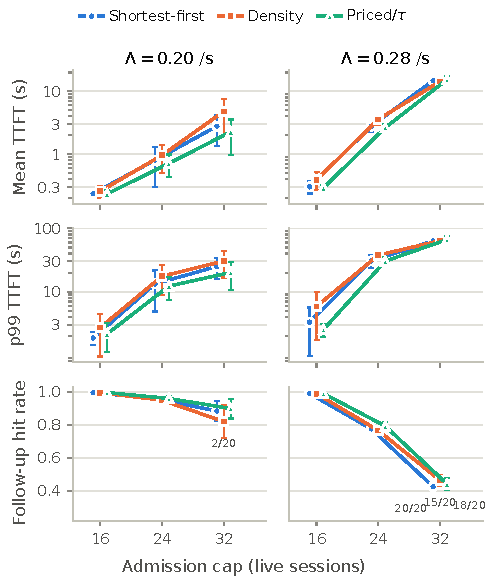
\includegraphics[width=\columnwidth]{sim/fig-admission}
\caption{Admission-cap sweep on the two-resource replica: mean and p99
time to first token and hit rate by cap and eviction rule at two session
arrival rates; annotations give the number of seeds (of 20) that
thrashed. Synthetic, uncalibrated.}
\label{fig:sim-admission}
\end{figure}

% Generated by `uv run python -m report.paper_tables` in
% validation/. Do not edit by hand.
\begin{table}[htbp]
\caption{Placement over 4 replicas with half of the new programs placed on replica~0 (the affinity node), follow-up turns of 5--15k-token contexts, state moved over one shared link of bandwidth $B$ (tokens/s) when that is cheaper than recomputing it. $x$: mean move cost over mean service; $\rho^*=x/(1+x)$, the inversion utilisation of Eq.~\eqref{eq:rhostar} for one node and an idle alternative; Inv.: the lowest program rate (per s, swept in steps of 0.05) at which always moving to the least-loaded replica beats affinity in mean turn response beyond both confidence intervals; $\rho_0$: utilisation of the affinity node at that rate; $\rho_L$: utilisation of the shared link under always-move there; mean turn response (s) of affinity, always-move and the lookahead rule of Eq.~\eqref{eq:lookahead}. The idle alternative gives the earliest inversion, so $\rho^*$ is a lower bound for any real alternative.}
\label{tab:sim-inversion}
\centering\scriptsize\setlength{\tabcolsep}{2pt}
\begin{tabular}{@{}ccccccccc@{}}
\toprule
$B$ & $x$ & $\rho^*$ & Inv. & $\rho_0$ & $\rho_L$ & Affinity & Move & Lookahead \\
\midrule
20000k & 0.01 & 0.01 & $\le 0.20$ & 0.13 & 0.00 & 0.082 & 0.072 & 0.072 \\
2000k & 0.08 & 0.08 & $\le 0.20$ & 0.13 & 0.00 & 0.082 & 0.074 & 0.072 \\
500k & 0.34 & 0.25 & 0.40 & 0.26 & 0.05 & 0.096 & 0.090 & 0.076 \\
125k & 1.32 & 0.57 & 1.60 & 0.98 & 0.96 & 4.621 & 0.983 & 0.120 \\
\bottomrule
\end{tabular}
\end{table}


\paragraph{Placement and a shared KV store.} Table~\ref{tab:sim-inversion}
takes Proposition~\ref{prop:routing} out of its model: four replicas
instead of one node and an idle alternative, a skewed placement that
loads one replica, and a state that is moved over one shared link
rather than recomputed, as a shared KV store would move it. The row
order is the proposition's: the faster the link, the cheaper the move
and the lower the load at which always moving beats strict affinity.
With a link that moves a context in a millisecond the inversion is
below the lowest load swept; with a link slower than a recompute it
sits near saturation. The utilisation of the affinity node at the
inversion follows $\rho^*$ for cheap moves and exceeds it for the
expensive one, because the link is itself a shared resource: at the
loads where a slow link would pay off, every program is moving and the
link saturates, which the single-node proposition does not see. The
lookahead rule, which moves only when the observed wait exceeds the
move cost, is below both at every load, so the choice a deployment
faces is not affinity or a store but how the store's transfer is priced
at decision time.

% Generated by `cargo run --release --example paper_tables` in
% libqueuingsim/. Do not edit by hand.
\begin{table}[t]
\caption{Replayed production sessions on the two-resource replica: 761 Claude Code sessions (26395 turns, mean final context 391k tokens, mean think time 23\,s) from the corpus of \S\ref{sec:exp-traces}, arriving Poisson at rate $\Lambda$ (per s), each played turn by turn; cost model with $K_c=a/b=50$k tokens, batch cap 8, eviction by price per byte-second, at most Cap live sessions (the rest wait to enter). Follow-up hit rate; the share of $\mathrm{Var}[S]$ of follow-up prefill work due to the hit/miss mixture (the rest is the spread of the appends) and the $\mathrm{CV}^2$ of that work; observed mean prefill wait $W_q$ and the PK wait from the measured $\lambda$, $\E[S]$, $\E[S^2]$ (s); mean TTFT (s). Entry waits of sessions held by the cap are in the data file. $\pm$ is a 95\,\% half-width over 5 seeds.}
\label{tab:sim-trace}
\centering\small\setlength{\tabcolsep}{2pt}
\begin{tabular}{@{}ccccccccc@{}}
\toprule
$\Lambda$ & Pool & Cap & Hit & Mix & $\mathrm{{CV}}^2$ & $W_q$ & PK & TTFT \\
\midrule
0.005 & $\infty$ & 24 & $1.00 \pm 0.00$ & 0.00 & 43.4 & 3 & 12 & 5 \\
0.005 & 4M & 8 & $0.92 \pm 0.10$ & 0.38 & 53.5 & 71 & 664 & 83 \\
0.005 & 4M & 16 & $0.74 \pm 0.35$ & 0.29 & 28.6 & 192 & 1954 & 206 \\
0.005 & 2M & 4 & $0.80 \pm 0.13$ & 0.59 & 8.1 & 66 & 703 & 91 \\
0.005 & 2M & 8 & $0.25 \pm 0.25$ & 0.18 & 1.9 & 302 & 5946 & 349 \\
0.005 & 1M & 2 & $0.86 \pm 0.09$ & 0.75 & 9.3 & 10 & 81 & 24 \\
0.005 & 1M & 4 & $0.51 \pm 0.12$ & 0.44 & 2.5 & 79 & 669 & 111 \\
0.010 & $\infty$ & 24 & $1.00 \pm 0.00$ & 0.00 & 35.2 & 9 & 36 & 11 \\
0.010 & 4M & 8 & $0.84 \pm 0.11$ & 0.41 & 22.1 & 133 & 1546 & 154 \\
0.010 & 4M & 16 & $0.28 \pm 0.20$ & 0.17 & 2.3 & 540 & 4093 & 578 \\
0.010 & 2M & 4 & $0.80 \pm 0.16$ & 0.58 & 9.7 & 66 & 706 & 92 \\
0.010 & 2M & 8 & $0.21 \pm 0.19$ & 0.16 & 1.7 & 315 & 5344 & 363 \\
0.010 & 1M & 2 & $0.86 \pm 0.09$ & 0.75 & 9.3 & 10 & 81 & 24 \\
0.010 & 1M & 4 & $0.50 \pm 0.11$ & 0.43 & 2.4 & 81 & 701 & 113 \\
\bottomrule
\end{tabular}
\end{table}


\paragraph{Replayed production sessions.} Table~\ref{tab:sim-trace}
replaces the synthetic classes by the production sessions of
\S\ref{sec:exp-traces}: sessions still arrive Poisson, but each one
replays a real session's appends, outputs, think times and length, so
the workload side of the model is measured and only the replica is
simulated. Three things follow. First, with no eviction every follow-up
turn hits and the prefill work still has
$\mathrm{CV}^2=\simTraceOpenCvMin$--$\simTraceOpenCvMax$, from the
appends alone; the mean TTFT is
\simTraceOpenTtftMin--\simTraceOpenTtftMax\,s at these loads because a
new session's first prompt, of a few hundred thousand tokens, is a
cold prefill that every turn behind it waits for. Second, once the pool
is finite the admission cap decides the regime. At the tight cap the
hit rate stays at or above \simTraceTightHitMin{} and the hit/miss
mixture supplies \simTraceTightMixMin--\simTraceTightMixMax\,\% of the
variance of follow-up prefill work, the split that E2 measures; at the
loose cap the replica thrashes, the hit rate falls to at most
\simTraceLooseHitMax{} and the mean TTFT exceeds
\simTraceLooseTtftMin\,s. The price of a tight cap is the entry wait,
up to \simTraceEntryMaxHours{} hours in the mean where the pool cannot
carry the offered sessions.
Third, the PK wait computed from the measured $\lambda$, $\E[S]$ and
$\E[S^2]$ of the prefill queue is above the observed wait in every cell,
by a factor of \simTracePkRatioMin{} to \simTracePkRatioMax. The live
sessions are a finite population of two to twenty-four, and a session
that is waiting cannot generate its next turn, so arrivals thin out as
the queue grows; the open M/G/1 queue of \S\ref{sec:batch} has no such
feedback and overstates the wait. The bracket of
Proposition~\ref{prop:price} is therefore conservative for small
populations, and E2 has to report the number of live sessions next to
the load.

\subsubsection{What the Simulation Does Not Show}\label{sec:sim-limits}

The simulator shares the model's abstractions. It does not model
block-level KV allocation beyond tail blocks, partial prefix hits
across sessions, collective-communication contention or a prefill
budget policy, and its replica has one capacity function for prefill
and decode. Its parameters were chosen to be plausible, not measured.
Its results show which decisions are robust to the assumptions we
dropped; they say nothing about how often each regime occurs in
practice. The experiments of \S\ref{sec:exp-real}, starting with the
calibration of E1, remain necessary.
.
% Every number comes from paper/sim/*.tex and every figure from
% paper/sim/fig-*.pdf, generated by
%   cd libqueuingsim && cargo run --release --example paper_tables
%   uv run ... python scripts/plot_sim.py
% scripts/check_sim.sh fails if the generated files are stale.
% ===========================================================================
% Generated by `uv run python -m report.paper_tables` in
% validation/. Do not edit by hand.
\newcommand{\simChecks}{35}
\newcommand{\simCalA}{0.194}
\newcommand{\simCalB}{6.51}
\newcommand{\simCalOmega}{0.057}
\newcommand{\simChecksPassed}{35}
\newcommand{\simDecodeShiftPct}{0.3}
\newcommand{\simEvictLruRatioMin}{1.0}
\newcommand{\simEvictLruRatioMax}{1.6}
\newcommand{\simEndUnknownHit}{0.59}
\newcommand{\simEndKnownHit}{1.00}
\newcommand{\simEndUnknownTtftRatio}{2.2}
\newcommand{\simPdAgree}{32}
\newcommand{\simPdCells}{32}
\newcommand{\simOffloadOk}{6}
\newcommand{\simOffloadCells}{6}
\newcommand{\simTracePkRatioMin}{4}
\newcommand{\simTracePkRatioMax}{12}
\newcommand{\simTraceOpenCvMin}{27}
\newcommand{\simTraceOpenCvMax}{38}
\newcommand{\simTraceOpenTtftMin}{62}
\newcommand{\simTraceOpenTtftMax}{208}
\newcommand{\simTraceTightHitMin}{0.59}
\newcommand{\simTraceTightReusedMin}{0.93}
\newcommand{\simTraceTightMixMin}{6}
\newcommand{\simTraceTightMixMax}{23}
\newcommand{\simTraceLooseHitMax}{0.66}
\newcommand{\simTraceLooseTtftMin}{966}
\newcommand{\simTraceSessions}{761}
\newcommand{\simTraceEntryMaxHours}{6}
\newcommand{\simPriceSmallRatioMin}{0.08}
\newcommand{\simPriceSmallRatioMax}{0.18}
\newcommand{\simPriceLargeRatioMin}{0.1}
\newcommand{\simPriceLargeRatioMax}{0.3}
\newcommand{\simPriceLiveMin}{2}
\newcommand{\simPriceLiveMax}{9}
\newcommand{\simPriceFiniteRatioMin}{3}
\newcommand{\simPriceFiniteRatioMax}{18}
\newcommand{\simPriceOverMin}{3}
\newcommand{\simPriceOverMax}{13}
\newcommand{\simPriceCapHolds}{every}
\newcommand{\simFiniteRatioMax}{4.5}
\newcommand{\simFiniteRatioMin}{1.09}
\newcommand{\simFiniteNMin}{2}
\newcommand{\simFiniteNMax}{64}
\newcommand{\simFiniteRho}{0.6}


\subsection{Uncalibrated Simulation}\label{sec:sim}

The propositions hold inside their model. This subsection asks two
further questions by discrete-event simulation: does a simulation that
satisfies a proposition's assumptions reproduce its closed form, and
when an assumption is dropped, does the decision the proposition implies
survive? The simulator is not calibrated. Its parameters are
illustrative, and every number below is a property of the simulated
model under a synthetic workload. None is a measurement of a serving
system, and none replaces an entry of \S\ref{sec:exp-real}.

\paragraph{Simulator.} \texttt{libqueuingsim} is an event-driven
simulator written in Rust with six models: an open G/G/$c$ FIFO queue,
cross-checked against Lindley's recursion; closed agent programs on a
single-turn replica with a finite KV pool; the two-resource replica of
\S\ref{sec:batch}, fed by Poisson sessions with the closed turn/tool
loop of \S\ref{sec:sessions}; offline eviction instances with an exact
dynamic-programming optimum; disaggregated pools (kept for a follow-up);
and replicas with per-program KV locality. The two-resource replica runs
iterations of length $\max(\omega+\beta K_B,\ n\,a)$ for a batch of $n$
decoding turns holding $K_B$ tokens of KV, so decode is a bandwidth PS
with the demand~\eqref{eq:decode} and prefill is a FIFO server that
receives the compute the batch leaves. Resident KV is a prefix; a turn
re-prefills what was evicted with the work~\eqref{eq:prefill}. We use
$a=2\cdot10^{-5}$, $b=2\cdot10^{-9}$, $\omega=2\cdot10^{-4}$ and, in
the open-session scenario, $\beta=2\cdot10^{-9}$ seconds per token.
Whether a program issues another turn is drawn when its tool call
returns, so a suspended program holds KV that may never be reused.

\paragraph{Checks.} Each proposition is a named check with fixed seeds
and an explicit tolerance. An \emph{in-model} check keeps the
proposition's assumptions, so a failure would indicate a bug in the
simulator or in the closed form. A \emph{beyond-model} check drops one:
a real batch cap, a hit rate that emerges from finite memory, or a
heuristic in place of the optimum. Offloading checks on the single-turn
replica are in the code but not shown; their one finding, that the
ranking of offloading policies flips with whether fetches hold the
replica, is recorded for E3. Of \simChecks{} checks,
\simChecksPassed{} pass. Confidence intervals are 95\,\% batch means or,
where stated, across independent seeds. Every table and figure in this
subsection is generated by the simulator from fixed seeds; the best
value in each comparison is in bold.

% Generated by `cargo run --release --example paper_tables` in
% libqueuingsim/. Do not edit by hand.
\begin{table}[t]
\caption{Simulation under each proposition's assumptions (in-model). M/M/1: $\mu=10$. PK: $\rho=0.7$. Cache: $\lambda=1.8$. SF/OPT: worst of 9000 instances with equal $p_i$. $\pm$ is a 95\,\% batch-means half-width. Times in seconds.}
\label{tab:sim-inmodel}
\centering\small
\begin{tabular}{@{}l@{\hspace{4pt}}lcc@{}}
\toprule
Quantity & Result & Theory & Simulated \\
\midrule
M/M/1 $W$, $\lambda=9$ & \S\ref{sec:intro} & 1.000 & $1.012 \pm 0.024$ \\
PK $W_q$, workload B & Thm.~\ref{thm:pk} & 4.002 & $3.960 \pm 0.052$ \\
$W_q^B/W_q^A$, $\rho=0.6$ & Prop.~\ref{prop:pk} & 3.43 & 3.42 \\
$\rho$ at $p=0.8$ & Prop.~\ref{prop:cache} & 0.252 & 0.253 \\
$W_q$ / M/M/1, $\mathrm{CV}^2{=}15.3$ & Eq.~\eqref{eq:cv2} & 8.15 & 8.10 \\
max SF/OPT & Prop.~\ref{prop:evict} & $\le 2$ & 1.791 \\
\bottomrule
\end{tabular}
\end{table}

% Generated by `cargo run --release --example paper_tables` in
% libqueuingsim/. Do not edit by hand.
\begin{table}[t]
\caption{Batching server under its assumptions (in-model): mean number of turns at the replica, $L=\lambda R$. Rows 1--4: Poisson turns at $\rho=0.7$, work deterministic or hit/miss ($0.05$\,s w.p.\ $0.8$, else $0.5$\,s; both mean $0.14$\,s); PS theory $\rho/(1-\rho)$, FIFO theory $\lambda W_q+\rho$. Rows 5--6: sessions arrive Poisson, each turn is followed by a tool call (mean 2\,s, $\mathrm{CV}^2=4$) and another turn w.p.\ $0.8$; theory $\sum_n n\pi(n)$ at $\lambda=\Lambda/(1-p)$ ($\rho=0.7$ for $\phi\equiv 1$, $\rho=3$ for $\phi(n)=n/(1+\beta(n-1))$). Row 7: rise of $L$ at a PS server when a fraction $\delta$ of turns becomes misses, hit rate $0.8$, $\rho=0.6$, against $[\lambda\delta\Phi_{\mathrm{PS}},\ \tfrac{C-\rho}{C-\rho'}\lambda\delta\Phi_{\mathrm{PS}}]$. Rows 8--9: the same misses on the two-resource replica (prefill FIFO in the compute left by a decode batch of $0.1$\,s per turn, mean availability $\bar r=0.96$): rise of the number in the prefill stage $L_P=\lambda\,\mathrm{TTFT}$ against the FIFO bracket at service $P/\bar r$, and of the number in the decode stage $L_D$, whose demand does not depend on hit or miss. $\pm$ is a 95\,\% batch-means half-width.}
\label{tab:sim-ps}
\centering\small\setlength{\tabcolsep}{3pt}
\begin{tabular}{@{}l@{\hspace{4pt}}lcc@{}}
\toprule
Quantity & Result & Theory & Simulated \\
\midrule
PS, D & \S\ref{sec:batch} & 2.333 & $2.338 \pm 0.021$ \\
PS, hit/miss & \S\ref{sec:batch} & 2.333 & $2.348 \pm 0.044$ \\
FIFO, D & Eq.~\eqref{eq:pk} & 1.517 & $1.519 \pm 0.011$ \\
FIFO, hit/miss & Eq.~\eqref{eq:pk} & 2.867 & $2.880 \pm 0.051$ \\
Loop, $\phi\equiv1$ & \S\ref{sec:sessions} & 2.33 & $2.36 \pm 0.07$ \\
Loop, sat.\ $\phi$ ($\beta{=}0.25$) & \S\ref{sec:sessions} & 12.00 & $12.32 \pm 0.39$ \\
PS $\Delta L$, $\delta{=}0.05$ & Prop.~\ref{prop:decode} & $[0.60,0.79]$ & $0.775 \pm 0.018$ \\
2-stage $\Delta L_P$, $\delta{=}0.05$ & Prop.~\ref{prop:price} & $[0.81,1.11]$ & $1.068 \pm 0.029$ \\
2-stage $\Delta L_D$, $\delta{=}0.05$ & Prop.~\ref{prop:decode} & 0 & $-0.000 \pm 0.000$ \\
\bottomrule
\end{tabular}
\end{table}


\subsubsection{In-Model: The Closed Forms}\label{sec:sim-inmodel}

Table~\ref{tab:sim-inmodel} compares the closed forms of
\S\ref{sec:congestion} and the price of a miss with simulation under
their own assumptions; the M/M/1 response time, the PK wait, the
variance ratio, the $(1+\mathrm{CV}^2)/2$ ratio of Eq.~\eqref{eq:cv2}
and the worst shortest-first ratio over 9000 instances agree with theory
within the confidence interval or 2\,\%. The $\Delta L$ row forces
misses on a fraction $\delta$ of turns at an M/G/1 server; the rise in
the number of turns lies inside the bracket of
Proposition~\ref{prop:price}(i), at its upper end where the exact PK
difference lies. Table~\ref{tab:sim-ps} does the same for the replica.
Under PS, deterministic and hit/miss work of equal mean give the same
occupancy, as insensitivity says, while a FIFO server separates them as
Eq.~\eqref{eq:pk} predicts. With Poisson sessions, a closed turn/tool
loop and hyperexponential tool times (the ``Loop'' rows), a PS replica
matches the isolated formula at the turn rate $\lambda=\Lambda/(1-p)$,
as the product form says. On the two-resource replica, forced misses
raise the prefill queue by an amount inside the bracket of
Proposition~\ref{prop:price} and leave the decode batch unchanged, as
Proposition~\ref{prop:decode} says; the prefill server's availability
was $0.96$ in this run, so the M/G/1 approximation of the prefill stage
is close. A Monte Carlo of the admission counts of
\S\ref{sec:batch} reproduces $2$, $7/4$, $1$ and $95/64$
to three decimals. These checks confirm the simulator, not the
propositions, which are already proved.

\subsubsection{Beyond the Model}\label{sec:sim-beyond}

% Generated by `uv run python -m report.paper_tables` in
% validation/. Do not edit by hand.
\begin{table}[htbp]
\caption{Batch cap $B=8$: exact limited PS (at most $B$ turns share $\phi(n)=n/(1+0.1(n-1))$, FIFO beyond) against PS with $\phi$ flattened at $B$, the model's approximation. Poisson turns, work of mean 1 with the given law ($\mathrm{CV}^2$ in brackets), load $u=\rho/\phi(B)$. Mean number at the replica; last column: relative error of the approximation for LPS, in \%. Mean response time has the same relative error (Little).}
\label{tab:sim-lps}
\centering\small\setlength{\tabcolsep}{3pt}
\begin{tabular}{@{}lccccc@{}}
\toprule
Work & $u$ & Formula & PS & LPS & Err. \\
\midrule
D (0) & 0.5 & 3.10 & $3.10 \pm 0.00$ & $3.08 \pm 0.00$ & $-1$ \\
D (0) & 0.8 & 7.33 & $7.33 \pm 0.06$ & $6.60 \pm 0.03$ & $-10$ \\
D (0) & 0.9 & 12.67 & $12.81 \pm 0.44$ & $9.90 \pm 0.22$ & $-22$ \\
Exp (1) & 0.5 & 3.10 & $3.11 \pm 0.01$ & $3.11 \pm 0.01$ & $+0$ \\
Exp (1) & 0.8 & 7.33 & $7.38 \pm 0.11$ & $7.38 \pm 0.11$ & $+1$ \\
Exp (1) & 0.9 & 12.67 & $12.73 \pm 0.52$ & $12.72 \pm 0.52$ & $+0$ \\
H2 (4) & 0.5 & 3.10 & $3.09 \pm 0.03$ & $3.12 \pm 0.03$ & $+1$ \\
H2 (4) & 0.8 & 7.33 & $7.29 \pm 0.18$ & $9.14 \pm 0.44$ & $+25$ \\
H2 (4) & 0.9 & 12.67 & $12.57 \pm 0.72$ & $20.31 \pm 1.87$ & $+60$ \\
\bottomrule
\end{tabular}
\end{table}


\paragraph{A real batch cap.} The model treats the batch limit $B$ by
flattening $\varphi$ at $B$, which keeps the decode stage insensitive. A
real cap admits turns beyond $B$ in FIFO order. Table~\ref{tab:sim-lps}
and Figure~\ref{fig:sim-lps} compare the two. At half load they agree
within 1\,\% for every work law, and for exponential work at every load.
At high load the error follows the work $\mathrm{CV}^2$: for
deterministic work the capped replica holds fewer turns than the formula
(by 22\,\% at $u=0.9$), for hyperexponential work with $\mathrm{CV}^2=4$
it holds more (by 51\,\%). A capped batch is not insensitive, and since
hit/miss work has $\mathrm{CV}^2>1$, the model underestimates decode
congestion at a capped replica near saturation. E1 and E2 must report
which regime a deployment is in.

\begin{figure}[t]
\centering
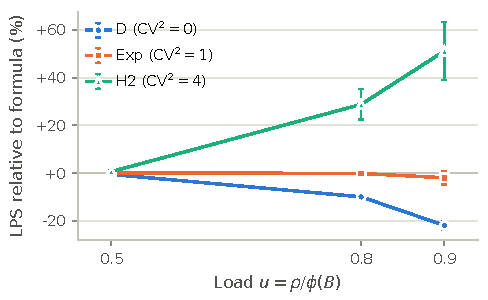
\includegraphics[width=\columnwidth]{sim/fig-lps}
\caption{Error of the saturating-$\varphi$ formula against an exact
batch cap ($B=8$) as a function of load, one line per work law. The
sign follows the work $\mathrm{CV}^2$. Synthetic, uncalibrated.}
\label{fig:sim-lps}
\end{figure}

% Generated by `cargo run --release --example paper_tables` in
% libqueuingsim/. Do not edit by hand.
\begin{table}[t]
\caption{Offline eviction: cost relative to the exact optimum of \eqref{eq:evict} with costs $p_ic_i^2$, over 3000 random instances per row (12 programs, $c_i\in\{1,\dots,200\}$, $\Delta C$ a random 10--60\,\% of the total).}
\label{tab:sim-evict}
\centering\small
\begin{tabular}{@{}lcccc@{}}
\toprule
Resume model & \multicolumn{2}{c}{SF mean / max} & \multicolumn{2}{c}{Density mean / max} \\
\midrule
equal $p_i$ & 1.108 & 1.67 & 1.108 & 1.67 \\
$p_i\sim U[0.05,1]$ & 1.902 & 10.05 & 1.136 & 2.86 \\
$p_i$ falls with $c_i$ & 2.037 & 8.60 & 1.146 & 2.67 \\
\bottomrule
\end{tabular}
\end{table}


\paragraph{Eviction offline.} Table~\ref{tab:sim-evict} and
Figure~\ref{fig:sim-evict} score eviction rules against the exact
optimum on random instances. With equal $p_i$, shortest-first and
price-per-byte order choose the same programs and stay within a factor
of~2 of the optimum, as Proposition~\ref{prop:blind}(ii) requires. When
$p_i$ varies, shortest-first reaches ten times the optimum and the
price-per-byte order stays close; the guarded rule of
Proposition~\ref{prop:guarded} is within $1.9$ of the optimum on every
instance and has the lowest mean in every row. With prices unrelated to
size, plain program-level order reaches $6.7$ times the optimum on
random instances, and the adversarial family of
Proposition~\ref{prop:guarded}(i) makes it arbitrarily bad. At block
granularity the threshold rule equals the optimum on every instance and
the density prefix plus one block never exceeds the optimum by more
than that block's price, as Proposition~\ref{prop:memory} states.

\begin{figure}[t]
\centering
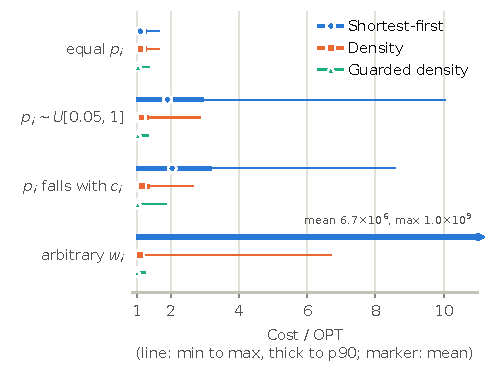
\includegraphics[width=\columnwidth]{sim/fig-evict-offline}
\caption{Offline eviction cost relative to the exact optimum by rule
and regime (mean, with the worst instance marked). Synthetic,
uncalibrated.}
\label{fig:sim-evict}
\end{figure}

% Generated by `uv run python -m report.paper_tables` in
% validation/. Do not edit by hand.
\begin{table}[htbp]
\caption{Eviction with open sessions on a replica with the vLLM~v1 engine's rules (those of Table~\ref{tab:sim-trace}) and the testbed's cost model. Sessions arrive Poisson at rate $\Lambda$ (per s): half agents ($p_i=0.95$, 4--8k initial tokens, tool calls Exp(6\,s)), half one-shot documents ($p_i=0.3$, 15--30k tokens, think time Exp(2\,s)); 600k-token KV, batch cap 8, at most 24 live sessions. Every policy evicts 16-token blocks from the tail of a context, sessions in a tool call before waiting ones (except LRU), and drops a finished session's blocks; rows marked $^*$ keep them, as vLLM's engine does, which cannot tell a finished session from one in a tool call. Throughput (turns/s), follow-up hit rate (the whole reusable prefix reused), mean and p99 time to first token (s), mean turn response (s; its half-width is in the data file), and the number of the 20 seeds that thrashed (follow-up turns reusing less than half of their reusable prefix); $\pm$ is a 95\,\% half-width over seeds; the best throughput, hit rate, TTFT and p99 per load in bold. Priced: $p_i\Phi_i/c_i$ with the FIFO price of Prop.~\ref{prop:price} from online estimates at the engine; Priced/$\tau$: per byte-second, $p_i\Phi_i/(c_i\tau_i)$ (the threshold rule of \S\ref{sec:evict}); Blocks: the same price of the tail block. The priced rules take $p_i$ and $\tau_i$ from the generating class (an oracle); the fixed keys see neither.}
\label{tab:sim-evict-dyn}
\centering\small\setlength{\tabcolsep}{2pt}
\begin{tabular}{@{}clcccccc@{}}
\toprule
$\Lambda$ & Policy & $X$ & Hit & TTFT & p99 & $R$ & Thr. \\
\midrule
0.03 & SF & \textbf{0.29} & \textbf{1.00} & $\mathbf{2.22 \pm 0.15}$ & \textbf{16.8} & 20.2 & 0 \\
0.03 & Density & \textbf{0.29} & \textbf{1.00} & $\mathbf{2.22 \pm 0.15}$ & \textbf{16.8} & 20.2 & 0 \\
0.03 & Priced & \textbf{0.29} & \textbf{1.00} & $\mathbf{2.22 \pm 0.15}$ & \textbf{16.8} & 20.2 & 0 \\
0.03 & Priced/$\tau$ & \textbf{0.29} & \textbf{1.00} & $\mathbf{2.22 \pm 0.15}$ & \textbf{16.8} & 20.2 & 0 \\
0.03 & Blocks & \textbf{0.29} & \textbf{1.00} & $\mathbf{2.22 \pm 0.15}$ & \textbf{16.8} & 20.2 & 0 \\
0.03 & LRU & \textbf{0.29} & \textbf{1.00} & $\mathbf{2.22 \pm 0.15}$ & \textbf{16.8} & 20.2 & 0 \\
0.03 & LRU$^*$ & \textbf{0.29} & \textbf{1.00} & $\mathbf{2.22 \pm 0.15}$ & \textbf{16.8} & 20.2 & 0 \\
0.03 & Priced/$\tau$$^*$ & \textbf{0.29} & 0.59 & $4.80 \pm 0.50$ & 29.3 & 23.6 & 0 \\
0.05 & SF & \textbf{0.38} & \textbf{0.83} & $34.45 \pm 1.01$ & 70.4 & 53.4 & 0 \\
0.05 & Density & \textbf{0.38} & \textbf{0.83} & $\mathbf{34.39 \pm 1.01}$ & \textbf{69.6} & 53.4 & 0 \\
0.05 & Priced & \textbf{0.38} & \textbf{0.83} & $34.48 \pm 0.99$ & 70.7 & 53.5 & 0 \\
0.05 & Priced/$\tau$ & \textbf{0.38} & \textbf{0.83} & $34.43 \pm 1.01$ & 70.4 & 53.4 & 0 \\
0.05 & Blocks & \textbf{0.38} & \textbf{0.83} & $34.46 \pm 1.00$ & 70.6 & 53.5 & 0 \\
0.05 & LRU & 0.27 & 0.75 & $56.41 \pm 1.76$ & 226.2 & 77.3 & 0 \\
0.05 & LRU$^*$ & 0.24 & 0.70 & $66.89 \pm 2.39$ & 240.9 & 88.2 & 0 \\
0.05 & Priced/$\tau$$^*$ & 0.35 & 0.45 & $41.73 \pm 0.68$ & 71.8 & 61.6 & 0 \\
\bottomrule
\end{tabular}
\end{table}

% Generated by `uv run python -m report.paper_tables` in
% validation/. Do not edit by hand.
\begin{table}[htbp]
\caption{Admission-cap sweep on the vLLM-rule replica: the scenario of Table~\ref{tab:sim-evict-dyn} with at most 16, 24 or 32 live sessions; later arrivals wait in an entry queue. Throughput (turns/s), follow-up hit rate, mean and p99 time to first token (s), mean turn response (s), mean entry-queue wait of a new session (s), and the number of the 20 seeds that thrashed. Means over seeds; the best throughput, hit rate, TTFT and p99 per ($\Lambda$, cap) in bold. The 95\,\% half-widths over seeds are the whiskers of Figure~\ref{fig:sim-admission}; Table~\ref{tab:sim-evict-dyn} states them for the rows it shares. An entry wait of hundreds of seconds means the replica does not carry the offered turn rate and the entry queue grows over the run; such values depend on the horizon (20\,000\,s). Every policy drops a finished session's blocks.}
\label{tab:sim-admission}
\centering\small\setlength{\tabcolsep}{2pt}
\begin{tabular}{@{}ccl@{\hspace{3pt}}cccccccc@{}}
\toprule
$\Lambda$ & Cap & Policy & $X$ & Hit & TTFT & p99 & $R$ & Entry & Thr. \\
\midrule
0.03 & 16 & SF & \textbf{0.29} & \textbf{1.00} & \textbf{2.21} & \textbf{16.5} & 20.20 & 0.1 & 0 \\
0.03 & 16 & Density & \textbf{0.29} & \textbf{1.00} & \textbf{2.21} & \textbf{16.5} & 20.20 & 0.1 & 0 \\
0.03 & 16 & Priced/$\tau$ & \textbf{0.29} & \textbf{1.00} & \textbf{2.21} & \textbf{16.5} & 20.20 & 0.1 & 0 \\
0.05 & 16 & SF & \textbf{0.41} & \textbf{1.00} & \textbf{14.54} & \textbf{33.5} & 32.89 & 1297.7 & 0 \\
0.05 & 16 & Density & \textbf{0.41} & \textbf{1.00} & \textbf{14.54} & \textbf{33.5} & 32.89 & 1297.7 & 0 \\
0.05 & 16 & Priced/$\tau$ & \textbf{0.41} & \textbf{1.00} & \textbf{14.54} & \textbf{33.5} & 32.89 & 1297.7 & 0 \\
0.03 & 24 & SF & \textbf{0.29} & \textbf{1.00} & \textbf{2.22} & \textbf{16.8} & 20.21 & 0.0 & 0 \\
0.03 & 24 & Density & \textbf{0.29} & \textbf{1.00} & \textbf{2.22} & \textbf{16.8} & 20.21 & 0.0 & 0 \\
0.03 & 24 & Priced/$\tau$ & \textbf{0.29} & \textbf{1.00} & \textbf{2.22} & \textbf{16.8} & 20.21 & 0.0 & 0 \\
0.05 & 24 & SF & \textbf{0.38} & \textbf{0.83} & 34.45 & 70.4 & 53.44 & 1407.5 & 0 \\
0.05 & 24 & Density & \textbf{0.38} & \textbf{0.83} & \textbf{34.39} & \textbf{69.6} & 53.38 & 1407.3 & 0 \\
0.05 & 24 & Priced/$\tau$ & \textbf{0.38} & \textbf{0.83} & 34.43 & 70.4 & 53.42 & 1408.4 & 0 \\
0.03 & 32 & SF & \textbf{0.29} & \textbf{1.00} & \textbf{2.22} & \textbf{16.8} & 20.21 & 0.0 & 0 \\
0.03 & 32 & Density & \textbf{0.29} & \textbf{1.00} & \textbf{2.22} & \textbf{16.8} & 20.21 & 0.0 & 0 \\
0.03 & 32 & Priced/$\tau$ & \textbf{0.29} & \textbf{1.00} & \textbf{2.22} & \textbf{16.8} & 20.21 & 0.0 & 0 \\
0.05 & 32 & SF & \textbf{0.32} & \textbf{0.57} & \textbf{64.01} & 144.5 & 84.49 & 1657.0 & 0 \\
0.05 & 32 & Density & \textbf{0.32} & \textbf{0.57} & 64.18 & \textbf{143.9} & 84.69 & 1659.3 & 0 \\
0.05 & 32 & Priced/$\tau$ & \textbf{0.32} & \textbf{0.57} & 64.10 & 145.1 & 84.58 & 1661.9 & 0 \\
\bottomrule
\end{tabular}
\end{table}


\paragraph{Open sessions and admission.} Tables~\ref{tab:sim-evict-dyn}
and~\ref{tab:sim-admission} and Figure~\ref{fig:sim-admission} run the
two-resource replica with Poisson sessions, half agents with long tool
calls and half one-shot documents with short think times, on a 600k-token
pool. Three things are visible. First, the price is paid in TTFT. The
p99 time to first token is ten to seventeen times its mean, because up
to eight admitted prefills queue behind a document miss, while turn
response exceeds TTFT by a constant decode time in every cell, as
Proposition~\ref{prop:decode} predicts; in this roofline model a batch
of eight is memory-bound and leaves prefill almost all of the compute.
Second, the byte-second key of Proposition~\ref{prop:memory}, which
drops documents with short think time and low resume probability first,
has the lowest TTFT and highest throughput of the priced rules in most
cells, but no cell separates it from shortest-first or from plain
price-per-byte order beyond the seed noise; LRU is worst everywhere, by
a factor of two or more in throughput. Third, admission decides more
than the eviction order. With at most 16 live sessions the hit rate
stays at $0.99$ and TTFT below $0.4$\,s at both loads; with 24 the hit
rate degrades to $0.77$ at the higher load; with 32 most seeds thrash
at the higher load, throughput falls by 40\,\% and TTFT reaches 15\,s.
The cost of a tight cap is the entry-queue wait, and at $\Lambda=0.28$
the replica does not carry the offered turn rate under any cap, so the
entry waits there are growth over the horizon, not steady state. The
simulation therefore points E4 at admission as much as at eviction, and
it suggests that the price of a state is dominated by the thrash it can
trigger, a transient effect outside the stationary
Propositions~\ref{prop:price} and~\ref{prop:decode}. These are
synthetic two-class results; we do not claim that they hold for real
traces.

\begin{figure}[t]
\centering
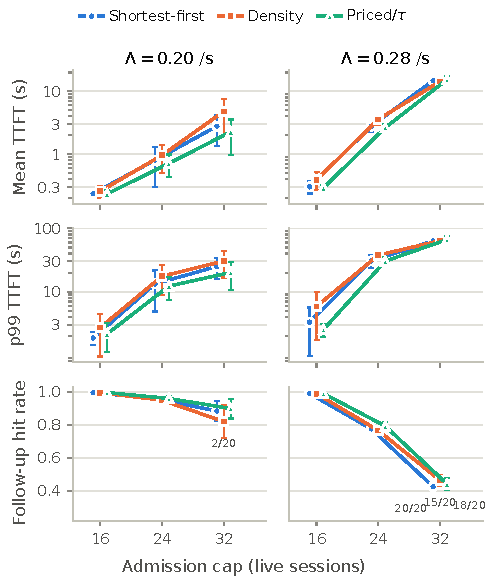
\includegraphics[width=\columnwidth]{sim/fig-admission}
\caption{Admission-cap sweep on the two-resource replica: mean and p99
time to first token and hit rate by cap and eviction rule at two session
arrival rates; annotations give the number of seeds (of 20) that
thrashed. Synthetic, uncalibrated.}
\label{fig:sim-admission}
\end{figure}

% Generated by `uv run python -m report.paper_tables` in
% validation/. Do not edit by hand.
\begin{table}[htbp]
\caption{Placement over 4 replicas with half of the new programs placed on replica~0 (the affinity node), follow-up turns of 5--15k-token contexts, state moved over one shared link of bandwidth $B$ (tokens/s) when that is cheaper than recomputing it. $x$: mean move cost over mean service; $\rho^*=x/(1+x)$, the inversion utilisation of Eq.~\eqref{eq:rhostar} for one node and an idle alternative; Inv.: the lowest program rate (per s, swept in steps of 0.05) at which always moving to the least-loaded replica beats affinity in mean turn response beyond both confidence intervals; $\rho_0$: utilisation of the affinity node at that rate; $\rho_L$: utilisation of the shared link under always-move there; mean turn response (s) of affinity, always-move and the lookahead rule of Eq.~\eqref{eq:lookahead}. The idle alternative gives the earliest inversion, so $\rho^*$ is a lower bound for any real alternative.}
\label{tab:sim-inversion}
\centering\scriptsize\setlength{\tabcolsep}{2pt}
\begin{tabular}{@{}ccccccccc@{}}
\toprule
$B$ & $x$ & $\rho^*$ & Inv. & $\rho_0$ & $\rho_L$ & Affinity & Move & Lookahead \\
\midrule
20000k & 0.01 & 0.01 & $\le 0.20$ & 0.13 & 0.00 & 0.082 & 0.072 & 0.072 \\
2000k & 0.08 & 0.08 & $\le 0.20$ & 0.13 & 0.00 & 0.082 & 0.074 & 0.072 \\
500k & 0.34 & 0.25 & 0.40 & 0.26 & 0.05 & 0.096 & 0.090 & 0.076 \\
125k & 1.32 & 0.57 & 1.60 & 0.98 & 0.96 & 4.621 & 0.983 & 0.120 \\
\bottomrule
\end{tabular}
\end{table}


\paragraph{Placement and a shared KV store.} Table~\ref{tab:sim-inversion}
takes Proposition~\ref{prop:routing} out of its model: four replicas
instead of one node and an idle alternative, a skewed placement that
loads one replica, and a state that is moved over one shared link
rather than recomputed, as a shared KV store would move it. The row
order is the proposition's: the faster the link, the cheaper the move
and the lower the load at which always moving beats strict affinity.
With a link that moves a context in a millisecond the inversion is
below the lowest load swept; with a link slower than a recompute it
sits near saturation. The utilisation of the affinity node at the
inversion follows $\rho^*$ for cheap moves and exceeds it for the
expensive one, because the link is itself a shared resource: at the
loads where a slow link would pay off, every program is moving and the
link saturates, which the single-node proposition does not see. The
lookahead rule, which moves only when the observed wait exceeds the
move cost, is below both at every load, so the choice a deployment
faces is not affinity or a store but how the store's transfer is priced
at decision time.

% Generated by `cargo run --release --example paper_tables` in
% libqueuingsim/. Do not edit by hand.
\begin{table}[t]
\caption{Replayed production sessions on the two-resource replica: 761 Claude Code sessions (26395 turns, mean final context 391k tokens, mean think time 23\,s) from the corpus of \S\ref{sec:exp-traces}, arriving Poisson at rate $\Lambda$ (per s), each played turn by turn; cost model with $K_c=a/b=50$k tokens, batch cap 8, eviction by price per byte-second, at most Cap live sessions (the rest wait to enter). Follow-up hit rate; the share of $\mathrm{Var}[S]$ of follow-up prefill work due to the hit/miss mixture (the rest is the spread of the appends) and the $\mathrm{CV}^2$ of that work; observed mean prefill wait $W_q$ and the PK wait from the measured $\lambda$, $\E[S]$, $\E[S^2]$ (s); mean TTFT (s). Entry waits of sessions held by the cap are in the data file. $\pm$ is a 95\,\% half-width over 5 seeds.}
\label{tab:sim-trace}
\centering\small\setlength{\tabcolsep}{2pt}
\begin{tabular}{@{}ccccccccc@{}}
\toprule
$\Lambda$ & Pool & Cap & Hit & Mix & $\mathrm{{CV}}^2$ & $W_q$ & PK & TTFT \\
\midrule
0.005 & $\infty$ & 24 & $1.00 \pm 0.00$ & 0.00 & 43.4 & 3 & 12 & 5 \\
0.005 & 4M & 8 & $0.92 \pm 0.10$ & 0.38 & 53.5 & 71 & 664 & 83 \\
0.005 & 4M & 16 & $0.74 \pm 0.35$ & 0.29 & 28.6 & 192 & 1954 & 206 \\
0.005 & 2M & 4 & $0.80 \pm 0.13$ & 0.59 & 8.1 & 66 & 703 & 91 \\
0.005 & 2M & 8 & $0.25 \pm 0.25$ & 0.18 & 1.9 & 302 & 5946 & 349 \\
0.005 & 1M & 2 & $0.86 \pm 0.09$ & 0.75 & 9.3 & 10 & 81 & 24 \\
0.005 & 1M & 4 & $0.51 \pm 0.12$ & 0.44 & 2.5 & 79 & 669 & 111 \\
0.010 & $\infty$ & 24 & $1.00 \pm 0.00$ & 0.00 & 35.2 & 9 & 36 & 11 \\
0.010 & 4M & 8 & $0.84 \pm 0.11$ & 0.41 & 22.1 & 133 & 1546 & 154 \\
0.010 & 4M & 16 & $0.28 \pm 0.20$ & 0.17 & 2.3 & 540 & 4093 & 578 \\
0.010 & 2M & 4 & $0.80 \pm 0.16$ & 0.58 & 9.7 & 66 & 706 & 92 \\
0.010 & 2M & 8 & $0.21 \pm 0.19$ & 0.16 & 1.7 & 315 & 5344 & 363 \\
0.010 & 1M & 2 & $0.86 \pm 0.09$ & 0.75 & 9.3 & 10 & 81 & 24 \\
0.010 & 1M & 4 & $0.50 \pm 0.11$ & 0.43 & 2.4 & 81 & 701 & 113 \\
\bottomrule
\end{tabular}
\end{table}


\paragraph{Replayed production sessions.} Table~\ref{tab:sim-trace}
replaces the synthetic classes by the production sessions of
\S\ref{sec:exp-traces}: sessions still arrive Poisson, but each one
replays a real session's appends, outputs, think times and length, so
the workload side of the model is measured and only the replica is
simulated. Three things follow. First, with no eviction every follow-up
turn hits and the prefill work still has
$\mathrm{CV}^2=\simTraceOpenCvMin$--$\simTraceOpenCvMax$, from the
appends alone; the mean TTFT is
\simTraceOpenTtftMin--\simTraceOpenTtftMax\,s at these loads because a
new session's first prompt, of a few hundred thousand tokens, is a
cold prefill that every turn behind it waits for. Second, once the pool
is finite the admission cap decides the regime. At the tight cap the
hit rate stays at or above \simTraceTightHitMin{} and the hit/miss
mixture supplies \simTraceTightMixMin--\simTraceTightMixMax\,\% of the
variance of follow-up prefill work, the split that E2 measures; at the
loose cap the replica thrashes, the hit rate falls to at most
\simTraceLooseHitMax{} and the mean TTFT exceeds
\simTraceLooseTtftMin\,s. The price of a tight cap is the entry wait,
up to \simTraceEntryMaxHours{} hours in the mean where the pool cannot
carry the offered sessions.
Third, the PK wait computed from the measured $\lambda$, $\E[S]$ and
$\E[S^2]$ of the prefill queue is above the observed wait in every cell,
by a factor of \simTracePkRatioMin{} to \simTracePkRatioMax. The live
sessions are a finite population of two to twenty-four, and a session
that is waiting cannot generate its next turn, so arrivals thin out as
the queue grows; the open M/G/1 queue of \S\ref{sec:batch} has no such
feedback and overstates the wait. The bracket of
Proposition~\ref{prop:price} is therefore conservative for small
populations, and E2 has to report the number of live sessions next to
the load.

\subsubsection{What the Simulation Does Not Show}\label{sec:sim-limits}

The simulator shares the model's abstractions. It does not model
block-level KV allocation beyond tail blocks, partial prefix hits
across sessions, collective-communication contention or a prefill
budget policy, and its replica has one capacity function for prefill
and decode. Its parameters were chosen to be plausible, not measured.
Its results show which decisions are robust to the assumptions we
dropped; they say nothing about how often each regime occurs in
practice. The experiments of \S\ref{sec:exp-real}, starting with the
calibration of E1, remain necessary.
.
% Every number comes from paper/sim/*.tex and every figure from
% paper/sim/fig-*.pdf, generated by
%   cd libqueuingsim && cargo run --release --example paper_tables
%   uv run ... python scripts/plot_sim.py
% scripts/check_sim.sh fails if the generated files are stale.
% ===========================================================================
% Generated by `uv run python -m report.paper_tables` in
% validation/. Do not edit by hand.
\newcommand{\simChecks}{35}
\newcommand{\simCalA}{0.194}
\newcommand{\simCalB}{6.51}
\newcommand{\simCalOmega}{0.057}
\newcommand{\simChecksPassed}{35}
\newcommand{\simDecodeShiftPct}{0.3}
\newcommand{\simEvictLruRatioMin}{1.0}
\newcommand{\simEvictLruRatioMax}{1.6}
\newcommand{\simEndUnknownHit}{0.59}
\newcommand{\simEndKnownHit}{1.00}
\newcommand{\simEndUnknownTtftRatio}{2.2}
\newcommand{\simPdAgree}{32}
\newcommand{\simPdCells}{32}
\newcommand{\simOffloadOk}{6}
\newcommand{\simOffloadCells}{6}
\newcommand{\simTracePkRatioMin}{4}
\newcommand{\simTracePkRatioMax}{12}
\newcommand{\simTraceOpenCvMin}{27}
\newcommand{\simTraceOpenCvMax}{38}
\newcommand{\simTraceOpenTtftMin}{62}
\newcommand{\simTraceOpenTtftMax}{208}
\newcommand{\simTraceTightHitMin}{0.59}
\newcommand{\simTraceTightReusedMin}{0.93}
\newcommand{\simTraceTightMixMin}{6}
\newcommand{\simTraceTightMixMax}{23}
\newcommand{\simTraceLooseHitMax}{0.66}
\newcommand{\simTraceLooseTtftMin}{966}
\newcommand{\simTraceSessions}{761}
\newcommand{\simTraceEntryMaxHours}{6}
\newcommand{\simPriceSmallRatioMin}{0.08}
\newcommand{\simPriceSmallRatioMax}{0.18}
\newcommand{\simPriceLargeRatioMin}{0.1}
\newcommand{\simPriceLargeRatioMax}{0.3}
\newcommand{\simPriceLiveMin}{2}
\newcommand{\simPriceLiveMax}{9}
\newcommand{\simPriceFiniteRatioMin}{3}
\newcommand{\simPriceFiniteRatioMax}{18}
\newcommand{\simPriceOverMin}{3}
\newcommand{\simPriceOverMax}{13}
\newcommand{\simPriceCapHolds}{every}
\newcommand{\simFiniteRatioMax}{4.5}
\newcommand{\simFiniteRatioMin}{1.09}
\newcommand{\simFiniteNMin}{2}
\newcommand{\simFiniteNMax}{64}
\newcommand{\simFiniteRho}{0.6}


\subsection{Uncalibrated Simulation}\label{sec:sim}

The propositions hold inside their model. This subsection asks two
further questions by discrete-event simulation: does a simulation that
satisfies a proposition's assumptions reproduce its closed form, and
when an assumption is dropped, does the decision the proposition implies
survive? The simulator is not calibrated. Its parameters are
illustrative, and every number below is a property of the simulated
model under a synthetic workload. None is a measurement of a serving
system, and none replaces an entry of \S\ref{sec:exp-real}.

\paragraph{Simulator.} \texttt{libqueuingsim} is an event-driven
simulator written in Rust with six models: an open G/G/$c$ FIFO queue,
cross-checked against Lindley's recursion; closed agent programs on a
single-turn replica with a finite KV pool; the two-resource replica of
\S\ref{sec:batch}, fed by Poisson sessions with the closed turn/tool
loop of \S\ref{sec:sessions}; offline eviction instances with an exact
dynamic-programming optimum; disaggregated pools (kept for a follow-up);
and replicas with per-program KV locality. The two-resource replica runs
iterations of length $\max(\omega+\beta K_B,\ n\,a)$ for a batch of $n$
decoding turns holding $K_B$ tokens of KV, so decode is a bandwidth PS
with the demand~\eqref{eq:decode} and prefill is a FIFO server that
receives the compute the batch leaves. Resident KV is a prefix; a turn
re-prefills what was evicted with the work~\eqref{eq:prefill}. We use
$a=2\cdot10^{-5}$, $b=2\cdot10^{-9}$, $\omega=2\cdot10^{-4}$ and, in
the open-session scenario, $\beta=2\cdot10^{-9}$ seconds per token.
Whether a program issues another turn is drawn when its tool call
returns, so a suspended program holds KV that may never be reused.

\paragraph{Checks.} Each proposition is a named check with fixed seeds
and an explicit tolerance. An \emph{in-model} check keeps the
proposition's assumptions, so a failure would indicate a bug in the
simulator or in the closed form. A \emph{beyond-model} check drops one:
a real batch cap, a hit rate that emerges from finite memory, or a
heuristic in place of the optimum. Offloading checks on the single-turn
replica are in the code but not shown; their one finding, that the
ranking of offloading policies flips with whether fetches hold the
replica, is recorded for E3. Of \simChecks{} checks,
\simChecksPassed{} pass. Confidence intervals are 95\,\% batch means or,
where stated, across independent seeds. Every table and figure in this
subsection is generated by the simulator from fixed seeds; the best
value in each comparison is in bold.

% Generated by `cargo run --release --example paper_tables` in
% libqueuingsim/. Do not edit by hand.
\begin{table}[t]
\caption{Simulation under each proposition's assumptions (in-model). M/M/1: $\mu=10$. PK: $\rho=0.7$. Cache: $\lambda=1.8$. SF/OPT: worst of 9000 instances with equal $p_i$. $\pm$ is a 95\,\% batch-means half-width. Times in seconds.}
\label{tab:sim-inmodel}
\centering\small
\begin{tabular}{@{}l@{\hspace{4pt}}lcc@{}}
\toprule
Quantity & Result & Theory & Simulated \\
\midrule
M/M/1 $W$, $\lambda=9$ & \S\ref{sec:intro} & 1.000 & $1.012 \pm 0.024$ \\
PK $W_q$, workload B & Thm.~\ref{thm:pk} & 4.002 & $3.960 \pm 0.052$ \\
$W_q^B/W_q^A$, $\rho=0.6$ & Prop.~\ref{prop:pk} & 3.43 & 3.42 \\
$\rho$ at $p=0.8$ & Prop.~\ref{prop:cache} & 0.252 & 0.253 \\
$W_q$ / M/M/1, $\mathrm{CV}^2{=}15.3$ & Eq.~\eqref{eq:cv2} & 8.15 & 8.10 \\
max SF/OPT & Prop.~\ref{prop:evict} & $\le 2$ & 1.791 \\
\bottomrule
\end{tabular}
\end{table}

% Generated by `cargo run --release --example paper_tables` in
% libqueuingsim/. Do not edit by hand.
\begin{table}[t]
\caption{Batching server under its assumptions (in-model): mean number of turns at the replica, $L=\lambda R$. Rows 1--4: Poisson turns at $\rho=0.7$, work deterministic or hit/miss ($0.05$\,s w.p.\ $0.8$, else $0.5$\,s; both mean $0.14$\,s); PS theory $\rho/(1-\rho)$, FIFO theory $\lambda W_q+\rho$. Rows 5--6: sessions arrive Poisson, each turn is followed by a tool call (mean 2\,s, $\mathrm{CV}^2=4$) and another turn w.p.\ $0.8$; theory $\sum_n n\pi(n)$ at $\lambda=\Lambda/(1-p)$ ($\rho=0.7$ for $\phi\equiv 1$, $\rho=3$ for $\phi(n)=n/(1+\beta(n-1))$). Row 7: rise of $L$ at a PS server when a fraction $\delta$ of turns becomes misses, hit rate $0.8$, $\rho=0.6$, against $[\lambda\delta\Phi_{\mathrm{PS}},\ \tfrac{C-\rho}{C-\rho'}\lambda\delta\Phi_{\mathrm{PS}}]$. Rows 8--9: the same misses on the two-resource replica (prefill FIFO in the compute left by a decode batch of $0.1$\,s per turn, mean availability $\bar r=0.96$): rise of the number in the prefill stage $L_P=\lambda\,\mathrm{TTFT}$ against the FIFO bracket at service $P/\bar r$, and of the number in the decode stage $L_D$, whose demand does not depend on hit or miss. $\pm$ is a 95\,\% batch-means half-width.}
\label{tab:sim-ps}
\centering\small\setlength{\tabcolsep}{3pt}
\begin{tabular}{@{}l@{\hspace{4pt}}lcc@{}}
\toprule
Quantity & Result & Theory & Simulated \\
\midrule
PS, D & \S\ref{sec:batch} & 2.333 & $2.338 \pm 0.021$ \\
PS, hit/miss & \S\ref{sec:batch} & 2.333 & $2.348 \pm 0.044$ \\
FIFO, D & Eq.~\eqref{eq:pk} & 1.517 & $1.519 \pm 0.011$ \\
FIFO, hit/miss & Eq.~\eqref{eq:pk} & 2.867 & $2.880 \pm 0.051$ \\
Loop, $\phi\equiv1$ & \S\ref{sec:sessions} & 2.33 & $2.36 \pm 0.07$ \\
Loop, sat.\ $\phi$ ($\beta{=}0.25$) & \S\ref{sec:sessions} & 12.00 & $12.32 \pm 0.39$ \\
PS $\Delta L$, $\delta{=}0.05$ & Prop.~\ref{prop:decode} & $[0.60,0.79]$ & $0.775 \pm 0.018$ \\
2-stage $\Delta L_P$, $\delta{=}0.05$ & Prop.~\ref{prop:price} & $[0.81,1.11]$ & $1.068 \pm 0.029$ \\
2-stage $\Delta L_D$, $\delta{=}0.05$ & Prop.~\ref{prop:decode} & 0 & $-0.000 \pm 0.000$ \\
\bottomrule
\end{tabular}
\end{table}


\subsubsection{In-Model: The Closed Forms}\label{sec:sim-inmodel}

Table~\ref{tab:sim-inmodel} compares the closed forms of
\S\ref{sec:congestion} and the price of a miss with simulation under
their own assumptions; the M/M/1 response time, the PK wait, the
variance ratio, the $(1+\mathrm{CV}^2)/2$ ratio of Eq.~\eqref{eq:cv2}
and the worst shortest-first ratio over 9000 instances agree with theory
within the confidence interval or 2\,\%. The $\Delta L$ row forces
misses on a fraction $\delta$ of turns at an M/G/1 server; the rise in
the number of turns lies inside the bracket of
Proposition~\ref{prop:price}(i), at its upper end where the exact PK
difference lies. Table~\ref{tab:sim-ps} does the same for the replica.
Under PS, deterministic and hit/miss work of equal mean give the same
occupancy, as insensitivity says, while a FIFO server separates them as
Eq.~\eqref{eq:pk} predicts. With Poisson sessions, a closed turn/tool
loop and hyperexponential tool times (the ``Loop'' rows), a PS replica
matches the isolated formula at the turn rate $\lambda=\Lambda/(1-p)$,
as the product form says. On the two-resource replica, forced misses
raise the prefill queue by an amount inside the bracket of
Proposition~\ref{prop:price} and leave the decode batch unchanged, as
Proposition~\ref{prop:decode} says; the prefill server's availability
was $0.96$ in this run, so the M/G/1 approximation of the prefill stage
is close. A Monte Carlo of the admission counts of
\S\ref{sec:batch} reproduces $2$, $7/4$, $1$ and $95/64$
to three decimals. These checks confirm the simulator, not the
propositions, which are already proved.

\subsubsection{Beyond the Model}\label{sec:sim-beyond}

% Generated by `uv run python -m report.paper_tables` in
% validation/. Do not edit by hand.
\begin{table}[htbp]
\caption{Batch cap $B=8$: exact limited PS (at most $B$ turns share $\phi(n)=n/(1+0.1(n-1))$, FIFO beyond) against PS with $\phi$ flattened at $B$, the model's approximation. Poisson turns, work of mean 1 with the given law ($\mathrm{CV}^2$ in brackets), load $u=\rho/\phi(B)$. Mean number at the replica; last column: relative error of the approximation for LPS, in \%. Mean response time has the same relative error (Little).}
\label{tab:sim-lps}
\centering\small\setlength{\tabcolsep}{3pt}
\begin{tabular}{@{}lccccc@{}}
\toprule
Work & $u$ & Formula & PS & LPS & Err. \\
\midrule
D (0) & 0.5 & 3.10 & $3.10 \pm 0.00$ & $3.08 \pm 0.00$ & $-1$ \\
D (0) & 0.8 & 7.33 & $7.33 \pm 0.06$ & $6.60 \pm 0.03$ & $-10$ \\
D (0) & 0.9 & 12.67 & $12.81 \pm 0.44$ & $9.90 \pm 0.22$ & $-22$ \\
Exp (1) & 0.5 & 3.10 & $3.11 \pm 0.01$ & $3.11 \pm 0.01$ & $+0$ \\
Exp (1) & 0.8 & 7.33 & $7.38 \pm 0.11$ & $7.38 \pm 0.11$ & $+1$ \\
Exp (1) & 0.9 & 12.67 & $12.73 \pm 0.52$ & $12.72 \pm 0.52$ & $+0$ \\
H2 (4) & 0.5 & 3.10 & $3.09 \pm 0.03$ & $3.12 \pm 0.03$ & $+1$ \\
H2 (4) & 0.8 & 7.33 & $7.29 \pm 0.18$ & $9.14 \pm 0.44$ & $+25$ \\
H2 (4) & 0.9 & 12.67 & $12.57 \pm 0.72$ & $20.31 \pm 1.87$ & $+60$ \\
\bottomrule
\end{tabular}
\end{table}


\paragraph{A real batch cap.} The model treats the batch limit $B$ by
flattening $\varphi$ at $B$, which keeps the decode stage insensitive. A
real cap admits turns beyond $B$ in FIFO order. Table~\ref{tab:sim-lps}
and Figure~\ref{fig:sim-lps} compare the two. At half load they agree
within 1\,\% for every work law, and for exponential work at every load.
At high load the error follows the work $\mathrm{CV}^2$: for
deterministic work the capped replica holds fewer turns than the formula
(by 22\,\% at $u=0.9$), for hyperexponential work with $\mathrm{CV}^2=4$
it holds more (by 51\,\%). A capped batch is not insensitive, and since
hit/miss work has $\mathrm{CV}^2>1$, the model underestimates decode
congestion at a capped replica near saturation. E1 and E2 must report
which regime a deployment is in.

\begin{figure}[t]
\centering
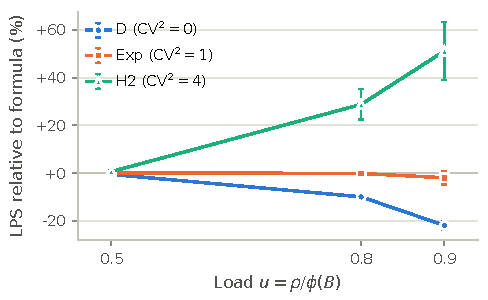
\includegraphics[width=\columnwidth]{sim/fig-lps}
\caption{Error of the saturating-$\varphi$ formula against an exact
batch cap ($B=8$) as a function of load, one line per work law. The
sign follows the work $\mathrm{CV}^2$. Synthetic, uncalibrated.}
\label{fig:sim-lps}
\end{figure}

% Generated by `cargo run --release --example paper_tables` in
% libqueuingsim/. Do not edit by hand.
\begin{table}[t]
\caption{Offline eviction: cost relative to the exact optimum of \eqref{eq:evict} with costs $p_ic_i^2$, over 3000 random instances per row (12 programs, $c_i\in\{1,\dots,200\}$, $\Delta C$ a random 10--60\,\% of the total).}
\label{tab:sim-evict}
\centering\small
\begin{tabular}{@{}lcccc@{}}
\toprule
Resume model & \multicolumn{2}{c}{SF mean / max} & \multicolumn{2}{c}{Density mean / max} \\
\midrule
equal $p_i$ & 1.108 & 1.67 & 1.108 & 1.67 \\
$p_i\sim U[0.05,1]$ & 1.902 & 10.05 & 1.136 & 2.86 \\
$p_i$ falls with $c_i$ & 2.037 & 8.60 & 1.146 & 2.67 \\
\bottomrule
\end{tabular}
\end{table}


\paragraph{Eviction offline.} Table~\ref{tab:sim-evict} and
Figure~\ref{fig:sim-evict} score eviction rules against the exact
optimum on random instances. With equal $p_i$, shortest-first and
price-per-byte order choose the same programs and stay within a factor
of~2 of the optimum, as Proposition~\ref{prop:blind}(ii) requires. When
$p_i$ varies, shortest-first reaches ten times the optimum and the
price-per-byte order stays close; the guarded rule of
Proposition~\ref{prop:guarded} is within $1.9$ of the optimum on every
instance and has the lowest mean in every row. With prices unrelated to
size, plain program-level order reaches $6.7$ times the optimum on
random instances, and the adversarial family of
Proposition~\ref{prop:guarded}(i) makes it arbitrarily bad. At block
granularity the threshold rule equals the optimum on every instance and
the density prefix plus one block never exceeds the optimum by more
than that block's price, as Proposition~\ref{prop:memory} states.

\begin{figure}[t]
\centering
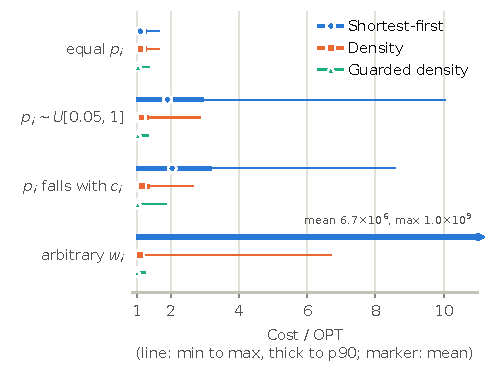
\includegraphics[width=\columnwidth]{sim/fig-evict-offline}
\caption{Offline eviction cost relative to the exact optimum by rule
and regime (mean, with the worst instance marked). Synthetic,
uncalibrated.}
\label{fig:sim-evict}
\end{figure}

% Generated by `uv run python -m report.paper_tables` in
% validation/. Do not edit by hand.
\begin{table}[htbp]
\caption{Eviction with open sessions on a replica with the vLLM~v1 engine's rules (those of Table~\ref{tab:sim-trace}) and the testbed's cost model. Sessions arrive Poisson at rate $\Lambda$ (per s): half agents ($p_i=0.95$, 4--8k initial tokens, tool calls Exp(6\,s)), half one-shot documents ($p_i=0.3$, 15--30k tokens, think time Exp(2\,s)); 600k-token KV, batch cap 8, at most 24 live sessions. Every policy evicts 16-token blocks from the tail of a context, sessions in a tool call before waiting ones (except LRU), and drops a finished session's blocks; rows marked $^*$ keep them, as vLLM's engine does, which cannot tell a finished session from one in a tool call. Throughput (turns/s), follow-up hit rate (the whole reusable prefix reused), mean and p99 time to first token (s), mean turn response (s; its half-width is in the data file), and the number of the 20 seeds that thrashed (follow-up turns reusing less than half of their reusable prefix); $\pm$ is a 95\,\% half-width over seeds; the best throughput, hit rate, TTFT and p99 per load in bold. Priced: $p_i\Phi_i/c_i$ with the FIFO price of Prop.~\ref{prop:price} from online estimates at the engine; Priced/$\tau$: per byte-second, $p_i\Phi_i/(c_i\tau_i)$ (the threshold rule of \S\ref{sec:evict}); Blocks: the same price of the tail block. The priced rules take $p_i$ and $\tau_i$ from the generating class (an oracle); the fixed keys see neither.}
\label{tab:sim-evict-dyn}
\centering\small\setlength{\tabcolsep}{2pt}
\begin{tabular}{@{}clcccccc@{}}
\toprule
$\Lambda$ & Policy & $X$ & Hit & TTFT & p99 & $R$ & Thr. \\
\midrule
0.03 & SF & \textbf{0.29} & \textbf{1.00} & $\mathbf{2.22 \pm 0.15}$ & \textbf{16.8} & 20.2 & 0 \\
0.03 & Density & \textbf{0.29} & \textbf{1.00} & $\mathbf{2.22 \pm 0.15}$ & \textbf{16.8} & 20.2 & 0 \\
0.03 & Priced & \textbf{0.29} & \textbf{1.00} & $\mathbf{2.22 \pm 0.15}$ & \textbf{16.8} & 20.2 & 0 \\
0.03 & Priced/$\tau$ & \textbf{0.29} & \textbf{1.00} & $\mathbf{2.22 \pm 0.15}$ & \textbf{16.8} & 20.2 & 0 \\
0.03 & Blocks & \textbf{0.29} & \textbf{1.00} & $\mathbf{2.22 \pm 0.15}$ & \textbf{16.8} & 20.2 & 0 \\
0.03 & LRU & \textbf{0.29} & \textbf{1.00} & $\mathbf{2.22 \pm 0.15}$ & \textbf{16.8} & 20.2 & 0 \\
0.03 & LRU$^*$ & \textbf{0.29} & \textbf{1.00} & $\mathbf{2.22 \pm 0.15}$ & \textbf{16.8} & 20.2 & 0 \\
0.03 & Priced/$\tau$$^*$ & \textbf{0.29} & 0.59 & $4.80 \pm 0.50$ & 29.3 & 23.6 & 0 \\
0.05 & SF & \textbf{0.38} & \textbf{0.83} & $34.45 \pm 1.01$ & 70.4 & 53.4 & 0 \\
0.05 & Density & \textbf{0.38} & \textbf{0.83} & $\mathbf{34.39 \pm 1.01}$ & \textbf{69.6} & 53.4 & 0 \\
0.05 & Priced & \textbf{0.38} & \textbf{0.83} & $34.48 \pm 0.99$ & 70.7 & 53.5 & 0 \\
0.05 & Priced/$\tau$ & \textbf{0.38} & \textbf{0.83} & $34.43 \pm 1.01$ & 70.4 & 53.4 & 0 \\
0.05 & Blocks & \textbf{0.38} & \textbf{0.83} & $34.46 \pm 1.00$ & 70.6 & 53.5 & 0 \\
0.05 & LRU & 0.27 & 0.75 & $56.41 \pm 1.76$ & 226.2 & 77.3 & 0 \\
0.05 & LRU$^*$ & 0.24 & 0.70 & $66.89 \pm 2.39$ & 240.9 & 88.2 & 0 \\
0.05 & Priced/$\tau$$^*$ & 0.35 & 0.45 & $41.73 \pm 0.68$ & 71.8 & 61.6 & 0 \\
\bottomrule
\end{tabular}
\end{table}

% Generated by `uv run python -m report.paper_tables` in
% validation/. Do not edit by hand.
\begin{table}[htbp]
\caption{Admission-cap sweep on the vLLM-rule replica: the scenario of Table~\ref{tab:sim-evict-dyn} with at most 16, 24 or 32 live sessions; later arrivals wait in an entry queue. Throughput (turns/s), follow-up hit rate, mean and p99 time to first token (s), mean turn response (s), mean entry-queue wait of a new session (s), and the number of the 20 seeds that thrashed. Means over seeds; the best throughput, hit rate, TTFT and p99 per ($\Lambda$, cap) in bold. The 95\,\% half-widths over seeds are the whiskers of Figure~\ref{fig:sim-admission}; Table~\ref{tab:sim-evict-dyn} states them for the rows it shares. An entry wait of hundreds of seconds means the replica does not carry the offered turn rate and the entry queue grows over the run; such values depend on the horizon (20\,000\,s). Every policy drops a finished session's blocks.}
\label{tab:sim-admission}
\centering\small\setlength{\tabcolsep}{2pt}
\begin{tabular}{@{}ccl@{\hspace{3pt}}cccccccc@{}}
\toprule
$\Lambda$ & Cap & Policy & $X$ & Hit & TTFT & p99 & $R$ & Entry & Thr. \\
\midrule
0.03 & 16 & SF & \textbf{0.29} & \textbf{1.00} & \textbf{2.21} & \textbf{16.5} & 20.20 & 0.1 & 0 \\
0.03 & 16 & Density & \textbf{0.29} & \textbf{1.00} & \textbf{2.21} & \textbf{16.5} & 20.20 & 0.1 & 0 \\
0.03 & 16 & Priced/$\tau$ & \textbf{0.29} & \textbf{1.00} & \textbf{2.21} & \textbf{16.5} & 20.20 & 0.1 & 0 \\
0.05 & 16 & SF & \textbf{0.41} & \textbf{1.00} & \textbf{14.54} & \textbf{33.5} & 32.89 & 1297.7 & 0 \\
0.05 & 16 & Density & \textbf{0.41} & \textbf{1.00} & \textbf{14.54} & \textbf{33.5} & 32.89 & 1297.7 & 0 \\
0.05 & 16 & Priced/$\tau$ & \textbf{0.41} & \textbf{1.00} & \textbf{14.54} & \textbf{33.5} & 32.89 & 1297.7 & 0 \\
0.03 & 24 & SF & \textbf{0.29} & \textbf{1.00} & \textbf{2.22} & \textbf{16.8} & 20.21 & 0.0 & 0 \\
0.03 & 24 & Density & \textbf{0.29} & \textbf{1.00} & \textbf{2.22} & \textbf{16.8} & 20.21 & 0.0 & 0 \\
0.03 & 24 & Priced/$\tau$ & \textbf{0.29} & \textbf{1.00} & \textbf{2.22} & \textbf{16.8} & 20.21 & 0.0 & 0 \\
0.05 & 24 & SF & \textbf{0.38} & \textbf{0.83} & 34.45 & 70.4 & 53.44 & 1407.5 & 0 \\
0.05 & 24 & Density & \textbf{0.38} & \textbf{0.83} & \textbf{34.39} & \textbf{69.6} & 53.38 & 1407.3 & 0 \\
0.05 & 24 & Priced/$\tau$ & \textbf{0.38} & \textbf{0.83} & 34.43 & 70.4 & 53.42 & 1408.4 & 0 \\
0.03 & 32 & SF & \textbf{0.29} & \textbf{1.00} & \textbf{2.22} & \textbf{16.8} & 20.21 & 0.0 & 0 \\
0.03 & 32 & Density & \textbf{0.29} & \textbf{1.00} & \textbf{2.22} & \textbf{16.8} & 20.21 & 0.0 & 0 \\
0.03 & 32 & Priced/$\tau$ & \textbf{0.29} & \textbf{1.00} & \textbf{2.22} & \textbf{16.8} & 20.21 & 0.0 & 0 \\
0.05 & 32 & SF & \textbf{0.32} & \textbf{0.57} & \textbf{64.01} & 144.5 & 84.49 & 1657.0 & 0 \\
0.05 & 32 & Density & \textbf{0.32} & \textbf{0.57} & 64.18 & \textbf{143.9} & 84.69 & 1659.3 & 0 \\
0.05 & 32 & Priced/$\tau$ & \textbf{0.32} & \textbf{0.57} & 64.10 & 145.1 & 84.58 & 1661.9 & 0 \\
\bottomrule
\end{tabular}
\end{table}


\paragraph{Open sessions and admission.} Tables~\ref{tab:sim-evict-dyn}
and~\ref{tab:sim-admission} and Figure~\ref{fig:sim-admission} run the
two-resource replica with Poisson sessions, half agents with long tool
calls and half one-shot documents with short think times, on a 600k-token
pool. Three things are visible. First, the price is paid in TTFT. The
p99 time to first token is ten to seventeen times its mean, because up
to eight admitted prefills queue behind a document miss, while turn
response exceeds TTFT by a constant decode time in every cell, as
Proposition~\ref{prop:decode} predicts; in this roofline model a batch
of eight is memory-bound and leaves prefill almost all of the compute.
Second, the byte-second key of Proposition~\ref{prop:memory}, which
drops documents with short think time and low resume probability first,
has the lowest TTFT and highest throughput of the priced rules in most
cells, but no cell separates it from shortest-first or from plain
price-per-byte order beyond the seed noise; LRU is worst everywhere, by
a factor of two or more in throughput. Third, admission decides more
than the eviction order. With at most 16 live sessions the hit rate
stays at $0.99$ and TTFT below $0.4$\,s at both loads; with 24 the hit
rate degrades to $0.77$ at the higher load; with 32 most seeds thrash
at the higher load, throughput falls by 40\,\% and TTFT reaches 15\,s.
The cost of a tight cap is the entry-queue wait, and at $\Lambda=0.28$
the replica does not carry the offered turn rate under any cap, so the
entry waits there are growth over the horizon, not steady state. The
simulation therefore points E4 at admission as much as at eviction, and
it suggests that the price of a state is dominated by the thrash it can
trigger, a transient effect outside the stationary
Propositions~\ref{prop:price} and~\ref{prop:decode}. These are
synthetic two-class results; we do not claim that they hold for real
traces.

\begin{figure}[t]
\centering
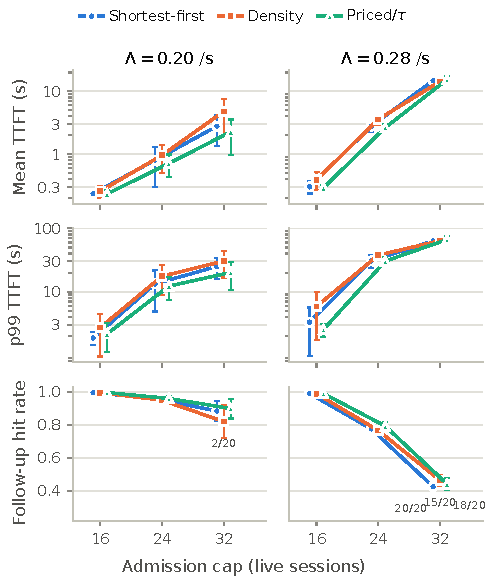
\includegraphics[width=\columnwidth]{sim/fig-admission}
\caption{Admission-cap sweep on the two-resource replica: mean and p99
time to first token and hit rate by cap and eviction rule at two session
arrival rates; annotations give the number of seeds (of 20) that
thrashed. Synthetic, uncalibrated.}
\label{fig:sim-admission}
\end{figure}

% Generated by `uv run python -m report.paper_tables` in
% validation/. Do not edit by hand.
\begin{table}[htbp]
\caption{Placement over 4 replicas with half of the new programs placed on replica~0 (the affinity node), follow-up turns of 5--15k-token contexts, state moved over one shared link of bandwidth $B$ (tokens/s) when that is cheaper than recomputing it. $x$: mean move cost over mean service; $\rho^*=x/(1+x)$, the inversion utilisation of Eq.~\eqref{eq:rhostar} for one node and an idle alternative; Inv.: the lowest program rate (per s, swept in steps of 0.05) at which always moving to the least-loaded replica beats affinity in mean turn response beyond both confidence intervals; $\rho_0$: utilisation of the affinity node at that rate; $\rho_L$: utilisation of the shared link under always-move there; mean turn response (s) of affinity, always-move and the lookahead rule of Eq.~\eqref{eq:lookahead}. The idle alternative gives the earliest inversion, so $\rho^*$ is a lower bound for any real alternative.}
\label{tab:sim-inversion}
\centering\scriptsize\setlength{\tabcolsep}{2pt}
\begin{tabular}{@{}ccccccccc@{}}
\toprule
$B$ & $x$ & $\rho^*$ & Inv. & $\rho_0$ & $\rho_L$ & Affinity & Move & Lookahead \\
\midrule
20000k & 0.01 & 0.01 & $\le 0.20$ & 0.13 & 0.00 & 0.082 & 0.072 & 0.072 \\
2000k & 0.08 & 0.08 & $\le 0.20$ & 0.13 & 0.00 & 0.082 & 0.074 & 0.072 \\
500k & 0.34 & 0.25 & 0.40 & 0.26 & 0.05 & 0.096 & 0.090 & 0.076 \\
125k & 1.32 & 0.57 & 1.60 & 0.98 & 0.96 & 4.621 & 0.983 & 0.120 \\
\bottomrule
\end{tabular}
\end{table}


\paragraph{Placement and a shared KV store.} Table~\ref{tab:sim-inversion}
takes Proposition~\ref{prop:routing} out of its model: four replicas
instead of one node and an idle alternative, a skewed placement that
loads one replica, and a state that is moved over one shared link
rather than recomputed, as a shared KV store would move it. The row
order is the proposition's: the faster the link, the cheaper the move
and the lower the load at which always moving beats strict affinity.
With a link that moves a context in a millisecond the inversion is
below the lowest load swept; with a link slower than a recompute it
sits near saturation. The utilisation of the affinity node at the
inversion follows $\rho^*$ for cheap moves and exceeds it for the
expensive one, because the link is itself a shared resource: at the
loads where a slow link would pay off, every program is moving and the
link saturates, which the single-node proposition does not see. The
lookahead rule, which moves only when the observed wait exceeds the
move cost, is below both at every load, so the choice a deployment
faces is not affinity or a store but how the store's transfer is priced
at decision time.

% Generated by `cargo run --release --example paper_tables` in
% libqueuingsim/. Do not edit by hand.
\begin{table}[t]
\caption{Replayed production sessions on the two-resource replica: 761 Claude Code sessions (26395 turns, mean final context 391k tokens, mean think time 23\,s) from the corpus of \S\ref{sec:exp-traces}, arriving Poisson at rate $\Lambda$ (per s), each played turn by turn; cost model with $K_c=a/b=50$k tokens, batch cap 8, eviction by price per byte-second, at most Cap live sessions (the rest wait to enter). Follow-up hit rate; the share of $\mathrm{Var}[S]$ of follow-up prefill work due to the hit/miss mixture (the rest is the spread of the appends) and the $\mathrm{CV}^2$ of that work; observed mean prefill wait $W_q$ and the PK wait from the measured $\lambda$, $\E[S]$, $\E[S^2]$ (s); mean TTFT (s). Entry waits of sessions held by the cap are in the data file. $\pm$ is a 95\,\% half-width over 5 seeds.}
\label{tab:sim-trace}
\centering\small\setlength{\tabcolsep}{2pt}
\begin{tabular}{@{}ccccccccc@{}}
\toprule
$\Lambda$ & Pool & Cap & Hit & Mix & $\mathrm{{CV}}^2$ & $W_q$ & PK & TTFT \\
\midrule
0.005 & $\infty$ & 24 & $1.00 \pm 0.00$ & 0.00 & 43.4 & 3 & 12 & 5 \\
0.005 & 4M & 8 & $0.92 \pm 0.10$ & 0.38 & 53.5 & 71 & 664 & 83 \\
0.005 & 4M & 16 & $0.74 \pm 0.35$ & 0.29 & 28.6 & 192 & 1954 & 206 \\
0.005 & 2M & 4 & $0.80 \pm 0.13$ & 0.59 & 8.1 & 66 & 703 & 91 \\
0.005 & 2M & 8 & $0.25 \pm 0.25$ & 0.18 & 1.9 & 302 & 5946 & 349 \\
0.005 & 1M & 2 & $0.86 \pm 0.09$ & 0.75 & 9.3 & 10 & 81 & 24 \\
0.005 & 1M & 4 & $0.51 \pm 0.12$ & 0.44 & 2.5 & 79 & 669 & 111 \\
0.010 & $\infty$ & 24 & $1.00 \pm 0.00$ & 0.00 & 35.2 & 9 & 36 & 11 \\
0.010 & 4M & 8 & $0.84 \pm 0.11$ & 0.41 & 22.1 & 133 & 1546 & 154 \\
0.010 & 4M & 16 & $0.28 \pm 0.20$ & 0.17 & 2.3 & 540 & 4093 & 578 \\
0.010 & 2M & 4 & $0.80 \pm 0.16$ & 0.58 & 9.7 & 66 & 706 & 92 \\
0.010 & 2M & 8 & $0.21 \pm 0.19$ & 0.16 & 1.7 & 315 & 5344 & 363 \\
0.010 & 1M & 2 & $0.86 \pm 0.09$ & 0.75 & 9.3 & 10 & 81 & 24 \\
0.010 & 1M & 4 & $0.50 \pm 0.11$ & 0.43 & 2.4 & 81 & 701 & 113 \\
\bottomrule
\end{tabular}
\end{table}


\paragraph{Replayed production sessions.} Table~\ref{tab:sim-trace}
replaces the synthetic classes by the production sessions of
\S\ref{sec:exp-traces}: sessions still arrive Poisson, but each one
replays a real session's appends, outputs, think times and length, so
the workload side of the model is measured and only the replica is
simulated. Three things follow. First, with no eviction every follow-up
turn hits and the prefill work still has
$\mathrm{CV}^2=\simTraceOpenCvMin$--$\simTraceOpenCvMax$, from the
appends alone; the mean TTFT is
\simTraceOpenTtftMin--\simTraceOpenTtftMax\,s at these loads because a
new session's first prompt, of a few hundred thousand tokens, is a
cold prefill that every turn behind it waits for. Second, once the pool
is finite the admission cap decides the regime. At the tight cap the
hit rate stays at or above \simTraceTightHitMin{} and the hit/miss
mixture supplies \simTraceTightMixMin--\simTraceTightMixMax\,\% of the
variance of follow-up prefill work, the split that E2 measures; at the
loose cap the replica thrashes, the hit rate falls to at most
\simTraceLooseHitMax{} and the mean TTFT exceeds
\simTraceLooseTtftMin\,s. The price of a tight cap is the entry wait,
up to \simTraceEntryMaxHours{} hours in the mean where the pool cannot
carry the offered sessions.
Third, the PK wait computed from the measured $\lambda$, $\E[S]$ and
$\E[S^2]$ of the prefill queue is above the observed wait in every cell,
by a factor of \simTracePkRatioMin{} to \simTracePkRatioMax. The live
sessions are a finite population of two to twenty-four, and a session
that is waiting cannot generate its next turn, so arrivals thin out as
the queue grows; the open M/G/1 queue of \S\ref{sec:batch} has no such
feedback and overstates the wait. The bracket of
Proposition~\ref{prop:price} is therefore conservative for small
populations, and E2 has to report the number of live sessions next to
the load.

\subsubsection{What the Simulation Does Not Show}\label{sec:sim-limits}

The simulator shares the model's abstractions. It does not model
block-level KV allocation beyond tail blocks, partial prefix hits
across sessions, collective-communication contention or a prefill
budget policy, and its replica has one capacity function for prefill
and decode. Its parameters were chosen to be plausible, not measured.
Its results show which decisions are robust to the assumptions we
dropped; they say nothing about how often each regime occurs in
practice. The experiments of \S\ref{sec:exp-real}, starting with the
calibration of E1, remain necessary.
